% ======================================================================
% Chinese integrated peer-review sidebar generated 14 July 2026.
% Review baseline and highlight locations remain those of 13 July 2026.
% Baseline: balloon511_ea_draft_en.pdf
% Manuscript text is unchanged; only PDF highlight annotations are added.
% Every annotation now contains its full Chinese finding and requested revision.
% Searchable Chinese source: ea_peer_review_report_cn_integrated_20260714.md.
% Round 1 colours: red major, orange moderate, blue structural, green journal.
% Round 2 (13 July 2026 (round 2, incremental)): additional highlights by author
% 'Peer reviewer - round 2'. Colours: violet new major, light violet new
% moderate, teal response to a round-1 item. IDs N01-N10 and Re-Mxx map
% to the round-2 addendum of the same HTML report.
% ======================================================================
\documentclass[11pt]{article}
\usepackage[a4paper,top=2.4cm,bottom=2.5cm,left=2.0cm,right=2.0cm]{geometry}
\usepackage{amsmath,amssymb,amsfonts}
\usepackage{fontspec}
\setmainfont{TeX Gyre Termes}
\usepackage{booktabs}
\usepackage{graphicx}
\graphicspath{{./}}
\usepackage[section]{placeins}
\renewcommand{\topfraction}{0.92}
\renewcommand{\bottomfraction}{0.8}
\renewcommand{\textfraction}{0.07}
\renewcommand{\floatpagefraction}{0.75}
\usepackage{xcolor}
\usepackage{tikz}
\usetikzlibrary{arrows.meta,positioning}
\usepackage{caption}
\captionsetup{font=small,labelfont=bf}
\usepackage{titlesec}
\titleformat{\section}{\normalfont\large\bfseries}{\thesection}{0.6em}{}
\titleformat{\subsection}{\normalfont\normalsize\bfseries}{\thesubsection}{0.5em}{}
\titleformat{\subsubsection}{\normalfont\normalsize\bfseries}{\thesubsubsection}{0.5em}{}
\titlespacing*{\section}{0pt}{1.3ex plus .2ex minus .2ex}{0.6ex}
\titlespacing*{\subsection}{0pt}{1.0ex plus .2ex minus .2ex}{0.5ex}
\usepackage{fancyhdr}
\pagestyle{fancy}
\fancyhf{}
\fancyhead[L]{\small\itshape Experimental Astronomy}
\fancyhead[R]{\small\thepage}
\renewcommand{\headrulewidth}{0.4pt}
\usepackage{cite}
\usepackage{hyperref}
\hypersetup{hidelinks,unicode=true}
\usepackage{pdfcomment}
% Highlight colours: red major, orange moderate, blue structural, green journal.

\setlength{\emergencystretch}{3em}
\newcommand{\keV}{\ensuremath{\,\mathrm{keV}}}
\newcommand{\MeV}{\ensuremath{\,\mathrm{MeV}}}
\newcommand{\cms}{\ensuremath{\,\mathrm{cm^{-2}\,s^{-1}}}}
\newcommand{\phcms}{\ensuremath{\,\mathrm{ph\,cm^{-2}\,s^{-1}}}}
\newcommand{\cps}{\ensuremath{\,\mathrm{s^{-1}}}}
\newcommand{\wii}{W_{511}}
\newcommand{\aeff}{A_{\mathrm{eff}}}
\newcommand{\fzero}{F_{0}}
\newcommand{\fthree}{F_{3\sigma}}
\raggedbottom

\begin{document}
\thispagestyle{fancy}
\begin{flushleft}
{\LARGE\bfseries \pdfmarkupcomment[markup=Highlight,color={0.62 0.86 0.62},author={中文同行审阅},subject={J02｜期刊｜摘要与图件}]{Detector-coupled Monte Carlo estimate of background and unresolved-line sensitivity for a balloon-borne 511 keV Laue-lens TES telescope}{【阅读说明】本文件以当前英文工作稿为左侧正文；每次修订后重新锚定仍有效的审阅意见，并生成对应的可见中文行动侧栏。第一轮正式条目 28 项、第二轮新增正式条目 10 项；原来没有行内锚点的 M06、M14、M15、M21、M22、J03 已补为零尺寸便笺。颜色：红色为重大问题，橙色为中等问题，蓝色为结构问题，绿色为期刊问题，紫色为第二轮新增，青色为第二轮复核。已完成全入射族活化的 M03 已从当前行动侧栏删除，其四处重复标注不再显示；M02 已在 2026-08-04 依据项目数据血缘更正并闭合，带状态的批注仅作修订追踪。 ｜ 【本处意见】本处标题过长，而且给人的灵敏度成熟度高于当前部分本底模型所能支持的程度；应缩短并明确范围。 ｜ 【正式问题】摘要长度和关键词数量合格，但结论强度与图件仍需修改 ｜ 【说明】摘要处于期刊 150–250 词范围内并有六个关键词，但 BGO 与 FWHM 未定义，完整性表述过强；多幅定量图仍为栅格图，稀疏谱图的图注也缺少可独立理解的归一化和不确定性说明。 ｜ 【修改要求】采用审阅报告给出的重写思路，定义缩写，并在缺失物理完成前保留范围限制句；图尽可能提供矢量 PDF/EPS，或满足线图/组合图分辨率要求；图注应补单位、箱宽、归一化状态和统计区间。 ｜ 【依据】本轮审阅时的 Experimental Astronomy 投稿指南 ｜ 【初始审阅定位页码】1, 5–20}\par}
\vspace{1.1em}
{\large Authors omitted for review\par}
\vspace{0.3em}
{\normalsize\itshape Affiliations omitted for review\par}
\end{flushleft}
\vspace{0.7em}
\noindent\rule{\textwidth}{0.4pt}
\vspace{0.5em}

\noindent\textbf{Abstract}\hspace{0.7em}
Background determines the sensitivity of a balloon-borne 511 keV Laue-lens
telescope with a transition-edge-sensor (TES) microcalorimeter. We developed an
end-to-end Geant4/MEGAlib model transporting focused signal, all eight prompt
families, production-position-sampled activation decays, and an explicit
atmospheric 511 keV line through one detector--cryostat geometry. All streams
share a $510.58$--$511.42\keV$ window, active anticoincidence, and
topology/field-of-view selection. In the mass-complete reference, the selected
prompt-plus-delayed diagnostic background was $(4.643\pm0.543)\times10^{-2}\cps$;
this differently scoped reference budget is used to locate sources, not as a
like-for-like measure of shield gain. Positrons and neutrons supplied
$96.8\%$ of the prompt component, and cold-copper $^{64}$Cu and $^{61}$Cu
accounted for 24 and two of 26 delayed records. This source map led to a
directionally graded BGO shield with 40, 30, and 10 mm side, bottom, and top
coverage and an open optical aperture. After a 420 eV FWHM pixel-level response
convolution, the active veto reduced the prompt rate from
$2.849\times10^{-2}$ to $4.072\times10^{-3}\cps$. \pdfmarkupcomment[markup=Highlight,color={0.85 0.74 0.98},author={中文同行审阅},subject={N08｜第二轮新增｜中等｜摘要可比性}]{Complete selection gave}{【7 月 14 日状态】当前摘要已明确参考数值是不同口径的瞬发加延迟来源诊断预算，不作为屏蔽增益的同口径比较；当前条目只保留核算边界问题。 ｜ 【本处意见】两套模拟现均为全入射族活化；剩余差别是参考预算不含显式大气线且用于来源诊断，而最终预算包含大气线并采用另一响应链。摘要须明确这不是纯屏蔽增益。 ｜ 【正式问题】摘要并列的参考率与最终率具有不同核算边界，不能解释为纯屏蔽增益 ｜ 【说明】当前两套模拟都已经完成全入射族活化输运；剩余问题是显示口径不同。参考几何数字用于瞬发加延迟的来源诊断，不含显式大气 511 keV 线；最终数字则包含瞬发、全八族延迟和大气线，并采用不同屏蔽与响应链。 ｜ 【修改要求】在摘要中明确前者是不同口径的来源诊断预算、不是同口径屏蔽增益；若要量化屏蔽增益，仍需给出相同源流、响应、阈值和选择下的成对计算。 ｜ 【依据】稿内摘要与方法口径 ｜ 【初始审阅定位页码】1}
background and signal rates of $6.965\times10^{-3}$ and
$9.862\times10^{-4}\cps$ at a top-of-atmosphere flux of $10^{-4}\phcms$. A
fixed-$45^\circ$-elevation, 20 d trajectory fold yielded a central counting
significance of 15.20 and a $3\sigma$ flux threshold of
$1.974\times10^{-5}\phcms$. The conditional component-wise transport-counting
endpoint gave 5.67 and $5.293\times10^{-5}\phcms$; it is a finite-transport
diagnostic, not full 95\% coverage.

\vspace{0.7em}
\noindent\textbf{Keywords}\hspace{0.7em}Gamma-ray instrumentation, 511 keV annihilation line, transition-edge sensors, Laue lens, balloon-borne telescope, activation background

\vspace{0.3em}
\noindent\rule{\textwidth}{0.4pt}
\vspace{1.0em}

\section{Introduction}
\label{sec:introduction}

Galactic 511 keV annihilation radiation is a direct observational probe of the
origin of Galactic positrons. Its spectrum contains a two-photon line near
511 keV and an ortho-positronium continuum at lower energy. Positrons annihilate
directly with electrons or form para-positronium, producing two photons near
511 keV, whereas ortho-positronium decays into a three-photon continuum. The
line intensity, profile, and positronium continuum therefore carry information
about the medium in which positrons slow down and annihilate
\cite{Prantzos2011,Jean2006}. The total Galactic 511 keV flux measured by
INTEGRAL/SPI corresponds, in an approximate steady state, to an annihilation
rate of a few $\times10^{43}\,\mathrm{e^+\,s^{-1}}$
\cite{Prantzos2011,Kierans2020}. Candidate positron sources include
$\beta^+$-unstable nuclei synthesized in stellar explosions, compact objects
that produce electron--positron pairs, and non-standard particle processes, but
the existing measurements do not uniquely identify the dominant channel
\cite{Prantzos2011,Siegert2016AA,Siegert2016V404}.

Wide-field observations have established the diffuse morphology of the line.
INTEGRAL/SPI finds a bright central bulge and a weaker disk, and a recent
20-year analysis recovers central, broad-bulge, and disk components while the
evidence for additional correlated structures remains marginal
\cite{Knodlseder2005AllSky,Siegert2016AA,Yoneda2025}. The 2016 COSI balloon flight independently
detected the bulge and found evidence that the emission is more extended than a
single point source \cite{Kierans2020,Siegert2020COSI}. Spectroscopy also
constrains the annihilation medium and kinematics: the SPI spectrum can be
decomposed into a narrow component with about $1.3\keV$ FWHM and a broad
component with about $5.4\keV$ FWHM, and spatial variations in centroid energy
and width have been sought across the inner Galaxy
\cite{Jean2006,Siegert2019Kinematics}. The annihilation map, however, records
where positrons slow down and annihilate, not necessarily where they were
created. Propagation through a magnetized, multiphase interstellar medium means
that diffuse morphology and spectroscopy alone cannot recover the dominant
source class or the complete pre-annihilation transport history
\cite{Prantzos2011}.

Wide-field Compton and coded-mask instruments are well suited to the total
bulge and disk emission. A complementary pointed instrument is needed to test
whether the central region also contains an unresolved central enhancement,
compact sources, or measurable line-kinematic structure. A detection of a
point-like or narrowly concentrated feature would show that part of the
annihilation is spatially localized; a non-detection would constrain a compact
component without excluding source populations whose positrons escape and
annihilate diffusely. An INTEGRAL/IBIS compact-source search found no Galactic
511 keV point sources and set a $2\sigma$ upper limit of about
$1.6\times10^{-4}\phcms$ for a $\sim10$ Ms Galactic-centre exposure
\cite{DeCesare2011}. This limit sets both the comparison scale of earlier
compact-source searches and a sensitivity target for a new narrow-field
pointing instrument.

Laue optics offer one route to such pointed observations by using
transmission-mode Bragg diffraction to focus photons from a known direction
onto a small focal plane \cite{Barriere2009Laue,Barriere2011LauePrototype}.
Concentrating the flux collected over a large aperture onto a smaller sensitive
detector area can improve point-source sensitivity when detector-related
background dominates \cite{Weidenspointner2006MAX}. The focal plane must then
combine a narrow energy response with sufficient stopping efficiency at
511 keV. Transition-edge-sensor (TES) microcalorimeters use the steep
resistive transition of a superconductor to measure small temperature changes
from deposited energy and can provide sub-keV resolution at 511 keV
\cite{Shirazi2023,Zhang2022TESGamma}. An array covers the focal spot, while thick absorbers and a
multilayer layout raise the full-energy efficiency. Laue focusing compresses
the accepted phase space, and the TES response permits a narrow line window and
detailed line-profile measurements.\vadjust{\smash{\hbox to 0pt{\pdfcomment[icon=Note,color={1 0.48 0.48},author={中文同行审阅},subject={M06｜重大｜科学用例｜补充正式条目}]{【本处意见】原标注 PDF 没有对应的行内高亮；现补充为相关位置的侧栏便笺。 ｜ 【正式问题】标题灵敏度只适用于未分辨的单色窄线 ｜ 【说明】科学动机讨论约 1.3 和 5.4 keV 的本征线宽，但信号为单色并用 ±0.420 keV 窗选择。高斯估算表明，该窗口可保留假定 0.420 keV 探测器线的约 98.1百分比，但卷积后对本征 FWHM 为 1.3 和 5.4 keV 的线仅保留约 53百分比 和 14.5百分比。 ｜ 【修改要求】报告灵敏度随本征线宽和质心偏移的优化结果，至少包括未分辨、1.3 keV 和 5.4 keV 三种情况；完成之前，每次引用阈值都应明确写“未分辨线”或“单色线”。 ｜ 【依据】依据稿内线宽所作的审阅者筛查计算 ｜ 【初始审阅定位页码】1–2, 9, 12, 20}\hss}}} The resulting instrument trades field of
view for a concentrated beam and high-resolution spectroscopy, complementing
rather than replacing wide-field bulge and disk measurements.

Focusing and energy resolution do not determine the useful sensitivity by
themselves because MeV line spectrometers are usually limited by local
instrumental background. Cosmic rays and atmospheric secondaries generate
prompt continua, local annihilation photons, and activation products that
accumulate with time in the detector and surrounding materials
\cite{Sturner2003,Gehrels1985}. Recent COSI work illustrates the required
analysis sequence: construct the transported payload mass model, separate
prompt and activation components, include anticoincidence, and connect the
result to the flight environment and its time variation
\cite{Kierans2017,Gallego2025Balloon,Gallego2025,Beechert2022,Sleator2019,Ciabattoni2025ACS}. The DIXE
TES background study likewise starts from a detailed payload model and explains
the detected spectrum by incident particle, production region, and physical
process \cite{Tian2026DIXE}. These studies show that the design question is not
only how much shielding surrounds the focal plane, but which directions and
materials generate the events that actually enter the science window.

We adopt the same source-to-detector approach. EXPACS/PARMA supplies the
balloon radiation field, and a 10 m Ge(111) Laue model supplies the focused
reference signal. Prompt particles, production-position-sampled activation
decays, an explicit atmospheric 511 keV line, and focused photons enter the
same generated detector--cryostat geometry and pass through the same response
and event selection. The analysis first identifies the dominant particle and
material origins of the background, then uses those origins to define the
final directionally graded active shield, and finally folds the selected signal
and background rates over a 20 d reference trajectory. This order connects the
background physics, the shield architecture, and the observing performance in
one traceable chain.

\subsection{Science and instrument requirements}
\label{sec:requirements}

The simulated instrument is aimed at 511 keV point-source or unresolved-central-excess components from the Galactic-center region that have not been detected by previous instruments. INTEGRAL/SPI measurements establish a sky dominated by diffuse bulge and disk emission \cite{Siegert2016AA,Yoneda2025}. The \pdfmarkupcomment[markup=Highlight,color={0.85 0.74 0.98},author={中文同行审阅},subject={N07｜第二轮新增｜中等｜引用支持}]{dedicated INTEGRAL/IBIS compact-source search}{【7 月 14 日状态】第 1.1 节以 IBIS 的 3σ 等效上限 2.4×10⁻⁴ ph cm⁻² s⁻¹ 乘 T=0.6520，得到唯一的载荷平面观测参考通量 1.565×10⁻⁴ ph cm⁻² s⁻¹；该数值不参与模拟归一化。 ｜ 【本处意见】本处以 IBIS 已发表 2σ 上限为依据，按高斯近似得到 3σ 等效上限 2.4×10⁻⁴ ph cm⁻² s⁻¹，再乘 T=0.6520，定义唯一的载荷平面观测参考通量 1.565×10⁻⁴ ph cm⁻² s⁻¹。 ｜ 【正式问题】SPI 的“10⁻⁴ 量级点源上限”被归给了弥散发射论文 ｜ 【说明】第 1.1 节原先把点状源通量上限归于弥散核球/盘分析；稿内唯一专门的紧致源检索是 INTEGRAL/IBIS（De Cesare 2011）。观测比较值还必须与蒙特卡洛归一化分开，不能把前者当成模拟输入。 ｜ 【修改要求】由 IBIS 紧致源检索单独承担观测依据：先将已发表的 2σ 上限按高斯近似线性换算为 3σ 等效上限 2.4×10⁻⁴ ph cm⁻² s⁻¹，再乘固定 45° 方向的大气透过率 0.6520，得到唯一的载荷平面观测参考通量 1.565×10⁻⁴ ph cm⁻² s⁻¹。 ｜ 【依据】引用范围核查；作者仍需对原始论文逐条确认 ｜ 【初始审阅定位页码】2} by De Cesare found no Galactic 511 keV point sources and reported a $2\sigma$ upper limit for a 10 Ms Galactic-center exposure \cite{DeCesare2011}. For comparison with the $3\sigma$ sensitivities reported here, we linearly rescale that published limit under the Gaussian approximation to obtain an IBIS-based $3\sigma$-equivalent above-atmosphere upper limit of $2.4\times10^{-4}\phcms$. At the day-15 altitude, the retained vertical residual depth is $3.461\,\mathrm{g\,cm^{-2}}$. For the fixed $45^\circ$-elevation axis the \pdfmarkupcomment[markup=Highlight,color={0.72 0.55 0.95},author={中文同行审阅},subject={N02｜第二轮新增｜重大｜信号透射几何}]{plane-parallel slant depth}{【7 月 14 日状态】已按固定 45° 仰角把垂直柱改为 √2 倍斜程柱：第 15 天 T=0.652034，并用同一规则重折叠全部 81 个时间箱；本条作为已实施修改的审阅追踪保留。 ｜ 【本处意见】本处现已写明 45° 平面平行斜程柱 4.895 g cm⁻² 和 T=0.6520；本条作为已完成修订的追踪保留。 ｜ 【正式问题】T=0.739 必须对应明确的剩余大气柱和视角；若把垂直柱用于 45° 侧向几何，信号约高估 12百分比 ｜ 【说明】T=0.739 对应 X≈3.5 g cm⁻² 的垂直剩余柱，这是 38.75 km 附近的典型量级；但光轴在地平线上方 45°，其斜程柱为垂直柱的 1.41 倍，对应 T≈0.65。稿件没有说明柱深、角度或衰减来源，同一 T-atm,511(t) 又乘到每个轨迹箱，错配会令整条信号曲线约降低 12百分比、通量阈值约升高 13百分比。 ｜ 【修改要求】说明 T=0.739 与 T-atm,511(t) 使用的大气柱、衰减数据源和视角；若锚点是垂直值，应按实际源仰角重算或给出理由。该项与 M05 的银河中心仰角问题直接耦合。 ｜ 【依据】标准大气柱与 XCOM 空气衰减的审阅者筛查计算 ｜ 【初始审阅定位页码】2, 9, 15} is $4.895\,\mathrm{g\,cm^{-2}}$; with an effective dry-air attenuation coefficient $0.08736\,\mathrm{cm^2\,g^{-1}}$, consistent with NIST XCOM near 511 keV, the transmission is $T_{15,45}=0.6520$. Applying this transmission defines the \pdfmarkupcomment[markup=Highlight,color={1 0.78 0.36},author={中文同行审阅},subject={M18｜中等｜通量约定}]{single payload-plane observational reference flux}{【7 月 14 日状态】第 1.1 节现仅以 IBIS 的 3σ 等效上限和 T=0.6520 定义唯一的载荷平面观测参考通量 1.565×10⁻⁴ ph cm⁻² s⁻¹；本段不再引入模拟归一化数值。 ｜ 【本处意见】本处只定义载荷平面的观测参考通量：2.4×10⁻⁴×0.6520=1.565×10⁻⁴ ph cm⁻² s⁻¹；不再在本段引入模拟注入通量及其载荷换算值。 ｜ 【正式问题】大气透射与有效面积术语不一致 ｜ 【说明】顶层大气通量乘以透射率 T 得到的是载荷处通量，而不是“载荷上方通量”。文中 S/F₀=11.13 cm² 已含 T=0.739，因此是包含大气的面积；按稿件定义，仪器本身的选择后面积约为 15.1 cm²。 ｜ 【修改要求】统一定义顶层大气和载荷处通量，说明天顶/斜程大气柱与透射模型，并把仪器有效面积与大气折叠后的计数—通量换算分开。 ｜ 【依据】稿内通量与面积定义 ｜ 【初始审阅定位页码】2, 9}, $F_{0,\mathrm{ref}}=(2.4\times10^{-4})\times0.6520=1.565\times10^{-4}\phcms$. This reference is used only to compare the reported sensitivity with the IBIS upper limit and is independent of the Monte Carlo signal normalization used later. Compared with the wide-field spectroscopic and coded-mask searches performed by INTEGRAL, the modeled payload adds Laue focusing to improve the point-source response and uses a high-energy-resolution, multilayer thick-absorber TES microcalorimeter array as the focal-plane detector to sharpen the 511 keV line measurement \cite{Shirazi2023,Caputo2017}.

This work first considers a balloon payload as an early test platform, with the expectation that the approach can later be extended to a satellite observing platform.

This goal imposes four requirements on the instrument and the simulation: first, the telescope must concentrate 511 keV photons collected by a large lens aperture onto a small focal plane, \pdfmarkupcomment[markup=Highlight,color={1 0.78 0.36},author={中文同行审阅},subject={M17｜中等｜探测器物理}]{increasing the collecting-area-to-detector-area ratio}{【7 月 14 日状态】正文保留单层约 49百分比 和六层接近 1 的原有简洁表述，仅将“探测效率”改为“相互作用效率”；同时已删除扩大天空立体角的表述。 ｜ 【本处意见】本处现准确表述聚焦收益为提高收集面积与探测器面积之比、降低探测器相关本底，并明确 Laue 透镜仍是窄视场定向光学，不再声称扩大天空覆盖。 ｜ 【正式问题】“探测效率”容易与系统探测效率混淆 ｜ 【说明】这里的单层约 49百分比 和六层接近 1 指 Ta 中发生相互作用的效率。 ｜ 【修改要求】仅将“探测效率”改为“相互作用效率”；本段无需追加其他效率解释。 ｜ 【依据】稿内探测效率术语 ｜ 【初始审阅定位页码】3} and reducing detector-associated background; this is a narrow-field pointed configuration rather than a means of increasing sky coverage. Second, the focal-plane detector must provide sub-keV energy response sufficient to resolve detailed line structure. Third, the detector and shield model must suppress atmospheric, activation, and side-entry backgrounds. Fourth, the simulation chain must treat prompt background, delayed activation, focused signal, vetoes, event topology, and mission-time variation consistently, so that signal and background are evaluated under the same detector selection.

The remainder of this paper is organized as follows. Section~\ref{sec:geometry} describes the detector and cryostat mass model; Section~\ref{sec:framework} the simulation framework---the workflow, optics coupling, background sources, event selection, and the mission-time trajectory fold (Section~\ref{sec:mission_time_fold}); Section~\ref{sec:results} the selected-rate and sensitivity results together with the normalization, convergence, and boundary checks; and Section~\ref{sec:discussion} the discussion and conclusions.

\section{Detector and cryostat mass model}
\label{sec:geometry}

The detector mass model is the generated, mass-complete Geant4/MEGAlib
reference geometry. It contains a balloon-borne multilayer TES array at the cold end of a
compact dilution refrigerator (DR), together with the thermal stages, magnetic
and passive shields, side-entry windows, collimator, copper thermal links,
active scintillator, and cryogenic service structures
\cite{Shirazi2023,Gottardi2021TESReview}. Figure~\ref{fig:mass_model} is rendered
directly from the semantic OBJ/MTL export of that generated geometry. The complete
view and the detector-bay view therefore show the model used for transport rather
than an idealized drawing.

The TES detector concept uses an absorber-coupled AlMn film structure developed in our laboratory; the advantages of AlMn alloy include transition-temperature tunability through composition and annealing, suitability for array fabrication, and relatively low magnetic-field sensitivity \cite{Xie2026AlMn,Vavagiakis2017AlMnMagnetic}. In the present concept, the TES thermometer film is an AlMn film of order $200\,\mathrm{nm}$ thickness, whereas the $\gamma$-ray absorber is a millimetre-scale metal body. The absorber uses $1.5\times1.5\times3.0\,\mathrm{mm^3}$ Ta pixels; the high atomic number of Ta increases the interaction efficiency for 511 keV photons. At 511 keV, a $3.0\,\mathrm{mm}$ Ta layer has an \pdfmarkupcomment[markup=Highlight,color={1 0.78 0.36},author={中文同行审阅},subject={M17｜中等｜探测器物理}]{estimated interaction efficiency of about}{【7 月 14 日状态】正文保留单层约 49百分比 和六层接近 1 的原有简洁表述，仅将“探测效率”改为“相互作用效率”；同时已删除扩大天空立体角的表述。 ｜ 【本处意见】本处仅作术语替换：单层约 49百分比 和六层接近 1 均称为相互作用效率，不追加其他效率解释。 ｜ 【正式问题】“探测效率”容易与系统探测效率混淆 ｜ 【说明】这里的单层约 49百分比 和六层接近 1 指 Ta 中发生相互作用的效率。 ｜ 【修改要求】仅将“探测效率”改为“相互作用效率”；本段无需追加其他效率解释。 ｜ 【依据】稿内探测效率术语 ｜ 【初始审阅定位页码】3} $49\%$, and the corresponding six-layer efficiency approaches unity. In the current geometry, the center-to-center spacing between adjacent Ta array layers is $12\,\mathrm{mm}$; this spacing is designed with the efficiency of the subsequent Compton-based kinematic-track veto mechanism in mind. The choice of Ta also considers its low-temperature low-specific-heat properties as a superconductor (this paper uses an order-of-magnitude estimate of $10^{-2}\,\mathrm{J\,K^{-1}\,m^{-3}}$) and a relatively high photoelectric-to-Compton interaction ratio; based on NIST XCOM cross sections near 511 keV, this ratio is about 0.731 \cite{NISTXCOM}. For the detector-response model, based on our laboratory experience with a previously developed X-ray TES \cite{Xie2026AlMn}, we adopt $\Delta E_{\mathrm{FWHM}}\simeq420\,\mathrm{eV}$ at 511 keV as an \pdfmarkupcomment[markup=Highlight,color={1 0.78 0.36},author={中文同行审阅},subject={M16｜中等｜探测器响应}]{estimated energy resolution and simulation input}{【7 月 14 日状态】正文已将 420 eV FWHM 简要标为预估能量分辨率和模拟响应输入，不再把它写成由热容证明的完整系统性能。 ｜ 【本处意见】本处现只简要说明 420 eV FWHM 是响应模型采用的预估能量分辨率，不再由热容推导或表述为已实测系统性能。 ｜ 【正式问题】420 eV 应明确标为预估能量分辨率 ｜ 【说明】当前探测器概念把 420 eV FWHM 作为逐像素高斯响应的输入；它不是探测效率，也不表述为完整阵列已经实测达到的性能。 ｜ 【修改要求】在正文中简要说明 420 eV FWHM 是响应模型采用的预估能量分辨率；具体响应实现仍在方法部分交代。 ｜ 【依据】稿内探测器响应定义 ｜ 【初始审阅定位页码】3, 10, 21}.

Because the TES film and Ta absorber differ greatly in size and mass, and because the TES film itself does not contribute significant 511 keV interactions, the transport geometry uses the Ta absorber to represent the main sensitive volume of a TES pixel. The explicit sensitive volume has six layers, 376 Ta absorber pixels per layer, and 2256 pixels in total, with 1.5 mm length and width and 3 mm thickness. A Si substrate proxy is placed below each Ta pixel, using Si to represent the SiO2-SiNx-Si substrate because this simulation does not model detailed thermal conduction. TES-film, wiring, and readout details are not built layer by layer as explicit interaction volumes; instead, they enter the model through the assumed energy response and service-mass proxies. Separately from the response FWHM, the retained W2 analysis selection uses the 511 keV line window W511 = 511 keV $\pm$ 420 eV, i.e. 510.58--511.42 keV.

The TES array is mounted on copper support and thermal-link structures. A copper
thermal finger passes through the rear of the sample box and joins the 50 mK
stage. The near-field box contains a 2 mm Nb inner magnetic shield and a 2 mm
MuMetal outer layer, represented as Ni:Fe = 4:1. Along the optical path, the
generated model contains 300 $\mu$m Al thermal-shield windows, a 25 $\mu$m Be
vacuum window, and an 8 mm W multihole collimator aligned with the TES pixels.
The side openings are Boolean cuts through every surrounding shell. The
reference geometry uses segmented CsI on the side and end surfaces; the
final optimized geometry replaces this outer active layer with BGO while leaving
the detector, cryostat, side aperture, and internal material layout unchanged.
The full instrument frame is rotated by $45^\circ$, so the local side window
points $45^\circ$ above the horizontal in the zenith-frame source coordinates.

The \pdfmarkupcomment[markup=Highlight,color={1 0.48 0.48},author={中文同行审阅},subject={M02｜重大｜审计更正（已闭合）}]{optimized BGO transport records shield hits}{【2026-08-04 审计更正】已由代码、原始 SIM 与生产目录闭合；不需要原生 50 keV 重跑。正文仅保留 50 keV 离线沉积能反符合的方法与硬件响应局限。 ｜ 【本处意见】【2026-08-04 审计更正】原始 SIM 与生产目录均保存低于 80 keV 的 CC HIT 沉积；最终选择按事例求和并离线施加 50 keV cut，因此无需原生阈值重跑。 ｜ 【正式问题】50 keV BGO 离线反符合的数据链完整 ｜ 【说明】2026-08-04 的项目数据血缘审计确认：最终定量选择只读取逐步 CC HIT 沉积，按事例累加匹配 BGO 主动体积的总沉积，并施加小于 50 keV 的后处理条件。原始 SIM 和生产目录均含低于 80 keV、包括 50–80 keV 的沉积；HTsim、原生 trigger/veto flag 及 detector map 中的 80 keV 字段均未参与最终选择。原审阅把 detector-map 字段推断为击中存储门的前提不成立。 ｜ 【修改要求】把正文中“记录与分析均为 50 keV”改成期刊化的方法描述：逐事例汇总主动屏蔽沉积，并施加 50 keV 离线沉积能反符合。无需原生阈值重跑；BGO 光学与电子学 turn-on 仍应作为独立的探测器响应局限。 ｜ 【依据】最终解析器与选择代码、原始 SIM 的 50–80 keV 沉积及生产 catalog 的数据血缘审计 ｜ 【初始审阅定位页码】4, 18, 21} with its native 80\keV{}
threshold, while the common detector-level selection applies the specified
50\keV{} shield-deposit veto to the recorded event information. Both values are
\pdfmarkupcomment[markup=Highlight,color={0.45 0.85 0.82},author={中文同行审阅},subject={Re-M02｜第二轮复核}]{kept fixed throughout the final-geometry calculation}{【第二轮复核】2026-08-04 的数据血缘审计推翻了本条第二轮推断：低于 80 keV 的 CC HIT 沉积已完整序列化，50–80 keV 事例可被 50 keV 离线 cut 正确否决。后续不得仅凭 detector-map 的 TriggerThreshold 字段推断分析记录门。}.

\begin{figure}[t]
\centering
\includegraphics[width=0.98\linewidth]{paper_source_figure_table/fig_reference_detector_cryostat_geometry.png}
\caption{Generated mass-complete reference geometry used in the detector transport.
(a) Complete detector--cryostat model, including the outer support frame,
active scintillator, cryostat stages, and service structures. (b) Detector-bay
view with the outer envelopes removed to expose the TES Ta array, copper thermal
link, side-window stack, and W collimator. The aperture axis points toward the
sky at $45^\circ$ elevation; the red arrow follows focused 511 keV photons from
the sky-facing collimator down to the TES array. Colours follow the semantic geometry export; selected
outer volumes are translucent only for visualization.}
\label{fig:mass_model}
\end{figure}

\FloatBarrier

\section{Simulation framework}
\label{sec:framework}

Detector-coupled Monte Carlo transport through detailed mass models is a mature method for predicting the response and background of gamma-ray spectrometers \cite{Sturner2003}. This section describes the full end-to-end simulation chain from source generation to flight-performance assessment.\vadjust{\smash{\hbox to 0pt{\pdfcomment[icon=Note,color={1 0.48 0.48},author={中文同行审阅},subject={M14｜重大｜可复现性｜补充正式条目}]{【本处意见】原标注 PDF 没有对应的行内高亮；现补充为相关位置的侧栏便笺。 ｜ 【正式问题】关键输运与响应配置缺失 ｜ 【说明】稿件未给出 Geant4、MEGAlib/Cosima、XOP/xoppylib/DABAX、PHITS/EXPACS 的精确版本，也未完整说明物理列表、电磁/强子模型、产生截断、放射性衰变设置、源能限/源面和大多数随机种子；数据声明只承诺将来建立仓库。 ｜ 【修改要求】投稿时归档并引用带版本的快照，纳入配置、几何与源文件、曝光表、轨迹数组、响应与选择代码、环境锁文件、种子以及可重建全部表图的脚本。 ｜ 【依据】稿内可复现性信息 ｜ 【初始审阅定位页码】6–9, 22}\hss}}} The focusing optics and detector system start from independent mass models: the optics-branch mass model takes the target point source and records focused photons reaching the \pdfmarkupcomment[markup=Highlight,color={0.48 0.72 1},author={中文同行审阅},subject={S02｜结构｜写作与行文}]{focal-plane plane}{【本处意见】删除重复词，改为 focal plane。 ｜ 【正式问题】文字可理解，但过于围绕开发过程且信息压缩过度 ｜ 【说明】若干段落把实现、理由、公式、验证和解释塞进超过 100 词的句子；“recording hook”“process class”“preregistered”“starved continuum”等内部开发用语，以及“easy to read”“three linked views”“two columns answer”等元话语削弱期刊文体。 ｜ 【修改要求】按科学功能拆分长句，删除起草/开发者旁白，直接陈述结果；统一 event/record/group/hit、分析窗术语、FoV 与 Laue 大小写，并统一美式或英式英语。 ｜ 【依据】全文写作与术语一致性 ｜ 【初始审阅定位页码】throughout} as the focused-source input to the detector branch; the detector branch then directly transports, in the detector/cryostat mass model of Section~\ref{sec:geometry}, prompt atmospheric particles, delayed decays generated from activation products according to recorded production positions, and the focused sources described above. The focused source, prompt source, and delayed source are simulated stepwise and normalized onto one time axis through Poisson-statistics-based time-axis sampling and renormalization, then the background is further suppressed by scintillator-based active veto and Compton-kinematics-based veto. The chain subsequently enters detailed background-analysis statistics, analysis of signal and background intensity variation caused by mission flight-time trajectory changes, and the overall flight-performance assessment and design-optimization recommendations. Because the focused signal and the two background streams all pass through the same response and veto definitions before any background decomposition or sensitivity statement, the subsequent results rest on a consistent event selection.

Figure~\ref{fig:workflow} expands this chain by computational layer: geometry definition, prompt and activation-accumulation transport, delayed-source construction, focused-optics transport, detector-coupled signal replay, veto mechanisms, detailed background analysis, time/flight-trajectory variation, and flight-performance assessment with design-optimization recommendations. The following subsections describe each layer's inputs, operations, and outputs.

Day-scale flights sample a continuum of altitude and geomagnetic states, so a single Monte Carlo snapshot cannot be linearly stretched in time. The mission-time trajectory fold---its motivation, analytic definitions, multi-point transport tests, and the resulting performance curves---is developed in Section~\ref{sec:mission_time_fold}.

\begin{figure}[t]
\centering
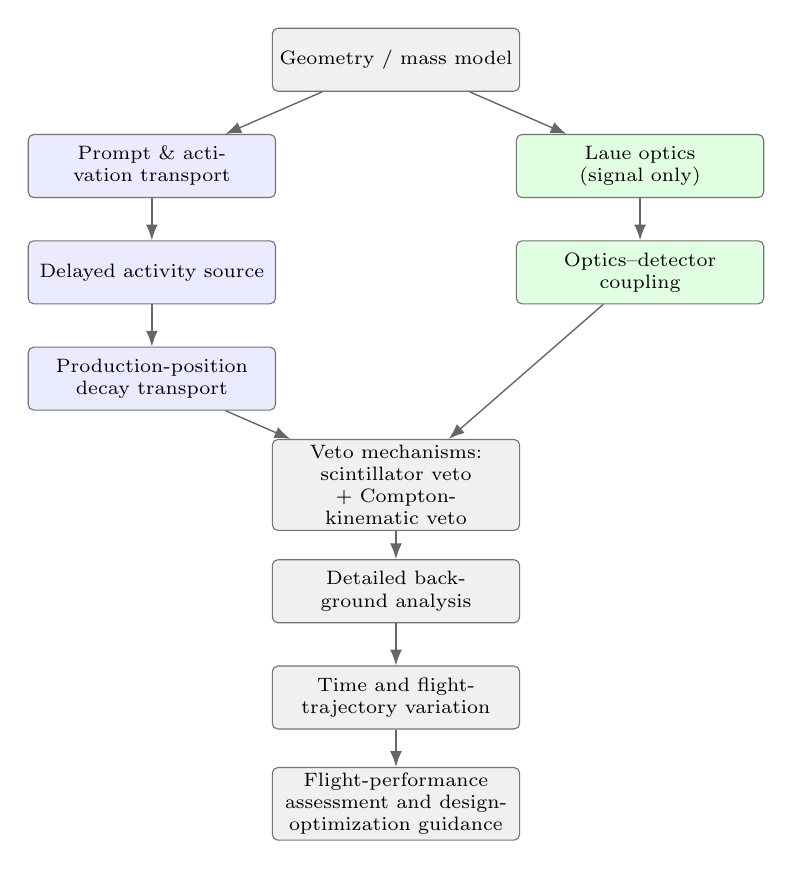
\begin{tikzpicture}[
  box/.style={rectangle, rounded corners=2pt, draw=black!55, line width=0.4pt,
              align=center, font=\scriptsize, text width=30mm, minimum height=8mm, inner sep=2pt},
  bg/.style={box, fill=blue!8},
  sig/.style={box, fill=green!12},
  shr/.style={box, fill=black!6},
  flow/.style={-{Latex[length=2mm]}, draw=black!60, line width=0.5pt}
]
\node[shr] (geo)    at (0,0)        {Geometry / mass model};
\node[bg]  (prompt) at (-3.1,-1.35) {Prompt \& activation transport};
\node[bg]  (delay)  at (-3.1,-2.7)  {Delayed activity source};
\node[bg]  (decay)  at (-3.1,-4.05) {Production-position decay transport};
\node[sig] (optics) at (3.1,-1.35)  {Laue optics (signal only)};
\node[sig] (couple) at (3.1,-2.7)   {Optics--detector coupling};
\node[shr] (sel)    at (0,-5.4)     {Veto mechanisms: scintillator veto $+$ Compton-kinematic veto};
\node[shr] (detail) at (0,-6.75)    {Detailed background analysis};
\node[shr] (fold)   at (0,-8.1)     {Time and flight-trajectory variation};
\node[shr] (out)    at (0,-9.45)    {Flight-performance assessment and design-optimization guidance};
\draw[flow] (geo) -- (prompt);
\draw[flow] (geo) -- (optics);
\draw[flow] (prompt) -- (delay);
\draw[flow] (delay) -- (decay);
\draw[flow] (optics) -- (couple);
\draw[flow] (decay) -- (sel);
\draw[flow] (couple) -- (sel);
\draw[flow] (sel) -- (detail);
\draw[flow] (detail) -- (fold);
\draw[flow] (fold) -- (out);
\end{tikzpicture}
\caption{Simulation chain used in this work. Blue nodes are the prompt and
delayed background streams, green nodes the focused-signal optics, and grey
nodes the shared geometry, veto mechanisms, detailed background analysis,
time/trajectory variation, and final flight-performance assessment. The focused
signal and all background streams are evaluated under the same detector response
and veto definitions before background decomposition, mission-time variation,
and design-optimization judgments are made.}
\label{fig:workflow}
\end{figure}

\FloatBarrier

\subsection{Laue optics and detector-coupled signal replay}
\label{sec:optics}

This simulation adopts a laue-lens system based on mosaic Ge(111) crystals \cite{Barriere2009Laue,Barriere2011LauePrototype}. Through optical design, it realizes a 10 m focal length, a 511\keV{} single-ring reference response, and an effective area of $20.1\,\mathrm{cm^2}$ at 511\keV; the effective area is calculated as
\begin{equation}
  A_{\mathrm{eff}}(E)=A_{\mathrm{inc}}\frac{N_{\mathrm{fp}}(E)}{N_{\mathrm{inc}}(E)}
  \label{eq:laue_aeff}
\end{equation}
where $A_{\mathrm{inc}}$ is the Monte Carlo incident sampling area, $N_{\mathrm{inc}}(E)$ is the number of incident photons, and $N_{\mathrm{fp}}(E)$ is the number of photons satisfying the focusing/focal-plane interception condition.
The \pdfmarkupcomment[markup=Highlight,color={1 0.48 0.48},author={中文同行审阅},subject={M08｜重大｜光学物理}]{mosaic system is adopted to make the Monte Carlo calculation convenient}{【本处意见】计算方便不是物理理由；应说明科学设计依据并验证响应。 ｜ 【正式问题】自定义 Laue 衍射过程需要晶片级物理验证 ｜ 【说明】把目标反射率转换成衍射平均自由程，再让标准吸收过程与之竞争，并不会自动重现原始反射率。稿件也未证明 XOP 镶嵌摇摆曲线与额外高斯晶面扰动是否重复计算角展宽，或是否正确抽样衍射微晶取向。所有信号和灵敏度结果都依赖这一响应。 ｜ 【修改要求】推导竞争风险构造；在角度和能量维度把反射、透射、吸收及出射角分布与 XOP/CRYSTAL 对比；证明步长收敛，并给出晶体尺寸、环几何、入射面积、模型版本和镶嵌抽样规则。 ｜ 【依据】稿内光学算法与验证链 ｜ 【初始审阅定位页码】5–6} while satisfying the expected focusing performance; other candidate schemes are also possible for actual engineering adaptation.

In this simulation, the laue optical branch gives the focusing-performance simulation and transports the focused signal through the Ge crystal mass.

For this purpose, the diffraction probability of photons by the crystal is no longer superposed onto photons as an efficiency parameter, but is defined as a discrete process at the Geant4 application layer \cite{Agostinelli2003,Allison2016}. The process takes the diffraction probability $R(|\Delta\theta|)$ according to the angular deviation of the current photon relative to the crystal plane, and converts it into a finite equivalent diffraction mean free path $\lambda_{\mathrm{diff}}$, so that the accumulated diffraction probability when the photon crosses a crystal path $\ell$ reproduces this value: $1-\exp(-\ell/\lambda_{\mathrm{diff}})=R(|\Delta\theta|)$, namely $\lambda_{\mathrm{diff}}=-\,\ell/\ln[1-R(|\Delta\theta|)]$; \pdfmarkupcomment[markup=Highlight,color={1 0.48 0.48},author={中文同行审阅},subject={M08｜重大｜光学物理}]{to avoid double counting with standard photoelectric absorption}{【本处意见】竞争过程构造不会自动重现目标 XOP 反射/透射/吸收；需给推导和晶片基准。 ｜ 【正式问题】自定义 Laue 衍射过程需要晶片级物理验证 ｜ 【说明】把目标反射率转换成衍射平均自由程，再让标准吸收过程与之竞争，并不会自动重现原始反射率。稿件也未证明 XOP 镶嵌摇摆曲线与额外高斯晶面扰动是否重复计算角展宽，或是否正确抽样衍射微晶取向。所有信号和灵敏度结果都依赖这一响应。 ｜ 【修改要求】推导竞争风险构造；在角度和能量维度把反射、透射、吸收及出射角分布与 XOP/CRYSTAL 对比；证明步长收敛，并给出晶体尺寸、环几何、入射面积、模型版本和镶嵌抽样规则。 ｜ 【依据】稿内光学算法与验证链 ｜ 【初始审阅定位页码】5–6}, $R$ is first normalized by the unabsorbed fraction ($R/(1-A)$) and then converted into a mean free path. After this mean free path is returned to Geant4, the diffraction process and the standard electromagnetic processes (photoelectric absorption and Compton scattering) \pdfmarkupcomment[markup=Highlight,color={0.45 0.85 0.82},author={中文同行审阅},subject={Re-M08｜第二轮复核}]{each sample interaction lengths in the same competition framework}{【第二轮复核】第二轮细化 M08：竞争框架中的首次相互作用概率为 LD/(LD+LA)×[1−exp(−(LD+LA))]；除弱吸收极限外，经 R/(1−A) 缩放后不会化为目标 R。XOP 镶嵌反射率已含微晶吸收和镶嵌宽度，额外高斯晶面扰动可能重复计算。应以 XOP 对比晶片 R/T/A 和出射角，并给出 A-inc。}, and the shortest one decides which process occurs first, rather than forcibly intercepting photons at the crystal boundary. Photons not selected to undergo diffraction still continue transport according to the standard electromagnetic physics, and may be absorbed, scattered, or directly transmitted.

The diffraction probability is preferentially given by interpolation in an external XOP/CRYSTAL rocking-curve map as a function of angular deviation: this curve is calculated offline once in the preprocessing stage by the CRYSTAL/diff\_pat module of the XOP toolkit (called through xoppylib, with DABAX crystallographic data as input) \cite{SanchezDelRio2011XOP}, and gives the Ge(111) reflectivity/transmissivity/absorption curves as a function of angular deviation; during transport, the angular deviation is calculated in real time for every step inside the crystal, and the current diffraction probability is obtained by interpolation on that curve, namely ``offline library tabulation, probability used by angle during transport''. The mosaic orientation is implemented by applying a Gaussian angular perturbation to the ideal Bragg-plane normal, with the perturbation width given by the 30 arcsec mosaic FWHM; after diffraction occurs, the outgoing direction is mirror-reflected according to the perturbed plane normal, and the photon energy is unchanged. This split in which the ``process class only handles the transport interface, and the independent model class handles probability and direction decisions'' follows the idea of existing crystal Bragg-reflection extensions in Geant4 \cite{Guan2023BraggReflection,Reiazi2025G4BraggReflection}, and extends it to the energy band needed here.

Here the reference signal is a monochromatic 511\keV{} point source whose
rounded top-of-atmosphere flux scale
($\fzero=10^{-4}\phcms$, Section~\ref{sec:requirements}) is motivated by the
dedicated INTEGRAL/IBIS compact-source upper limit \cite{DeCesare2011}, rather
than by any single observed object. It is constructed as a MEGAlib far-field source
\cite{Zoglauer2006}, with the detailed construction given in
Section~\ref{subsec:pointsource}. The signal is transported through the optics
branch and injected into the detector mass model as a parallel-beam source;
prompt cosmic-ray background and activation decays are transported directly in
the detector/cryostat mass model. The \pdfmarkupcomment[markup=Highlight,color={1 0.48 0.48},author={中文同行审阅},subject={M01｜重大｜科学范围}]{primary background budget}{【本处意见】这里明确排除了光学系统和其他载荷质量，因此任务级总本底表述必须收窄，或先输运/约束遗漏贡献。 ｜ 【正式问题】报告的本底只覆盖探测器—低温恒温器子系统，而非完整载荷 ｜ 【说明】论文把几何称为质量完备、把流程称为端到端，但本底预算明确只覆盖探测器—低温恒温器分支。Laue 透镜、透镜支撑、吊舱及其他载荷质量都可能散射辐射并产生瞬发或活化产物；在输运或约束这些贡献之前，不能据此推断任务级总本底。 ｜ 【修改要求】要么在包含光学系统和主要支撑质量的载荷模型中输运全部本底族，要么给出有依据的上限。完成之前，标题、摘要、结果和结论应统一使用“探测器—低温恒温器子系统本底”。 ｜ 【依据】稿内范围与表述的一致性 ｜ 【初始审阅定位页码】6, 21} is therefore
defined for the detector/cryostat branch, while the optics branch supplies the
transported focal-plane signal phase space.

\subsection{Source construction}
\label{sec:background}

After the focusing optics have been defined in Section~\ref{sec:optics}, the
optical input and the subsequent detector input \pdfmarkupcomment[markup=Highlight,color={0.72 0.55 0.95},author={中文同行审阅},subject={N03｜第二轮新增｜重大｜源流记账}]{require three source layers}{【本处意见】摘要承诺四个流且大气线占 26.59百分比，这里却只有三层、表 1 只有三项、符合轴也只有瞬发/延迟/信号；需说明第四流在哪里进入以及表 5 两列如何产生。 ｜ 【正式问题】第四个本底流缺失于源枚举、源表和公共时间轴 ｜ 【说明】摘要和引言承诺信号、瞬发、延迟与大气 511 keV 线四个输入共享同一选择，且大气线占最终本底 26.59百分比；但第 3.2 节只构造“三个源层”，表 1 只列三个，第 3.4.1 节时间轴也只有瞬发/延迟/信号。大气线似乎绕开了文档化的泊松轴、偶然符合和反符合机制，直到最终 cut-flow 才出现八条记录。 ｜ 【修改要求】把该流加入第 3.2 节、表 1 和公共时间轴，并补齐 M04 要求的来源与归一化；若它确实不经过公共轴，则必须明确解释表 5 的主动反符合和拓扑列如何生成。 ｜ 【依据】稿内源流枚举与 cut-flow ｜ 【初始审阅定位页码】1, 6, 8, 11, 19}: the
prompt atmospheric particle field incident on the payload, the delayed
radioactive population accumulated in the instrument by that particle field, and
the reference signal point source. These three layers are constructed
separately, rather than running transport by directly invoking MEGAlib's buildup
function for them at the same time, to reduce computational cost.

\subsubsection{Prompt atmospheric source}
\label{subsec:prompt_source}

The prompt atmospheric field is derived from EXPACS/PARMA. \pdfmarkupcomment[markup=Highlight,color={1 0.78 0.36},author={中文同行审阅},subject={M19｜中等｜源归一化}]{PARMA3.0}{【本处意见】应区分 PARMA 能谱模型版本与所引天顶角扩展，并记录准确 EXPACS 版本。 ｜ 【正式问题】PARMA 模型版本与角分布/源面归一化需要分开说明 ｜ 【说明】源段落称 PARMA3.0，却引用与 4.0 版相关的 2016 天顶角扩展；从等 μ 分箱方向强度到远场面积源速率的换算也未完整定义，尤其缺少投影面积因子和曝光单位。 ｜ 【修改要求】区分能谱模型和角分布模型版本，公开微分通量单位与源面约定，并推导含立体角和投影面积因子的分箱积分速率。 ｜ 【依据】稿内模型版本和归一化定义 ｜ 【初始审阅定位页码】6–7} is an
analytical model parameterized from PHITS atmospheric-shower calculations and
benchmarked against terrestrial cosmic-ray measurements, and EXPACS is its
public tabulation and software interface
\cite{Sato2015EXPACS,Sato2016PARMA4}. PHITS supplies the underlying
particle-transport physics: primary cosmic rays interact with air nuclei, the
secondary hadrons, leptons, photons, and neutrons are transported through the
atmospheric column, and the resulting fluences are parameterized by altitude,
geomagnetic cutoff, solar modulation, energy, and direction. In this work
EXPACS/PARMA provides the differential incident flux as a function of particle
species, kinetic energy, zenith angle, geographic position, altitude, cutoff
rigidity, and solar activity, and is used only to construct the external
radiation fields; detector response, vetoing, topology selection, and
mission-time counting are applied downstream. The reference source definitions
use latitude $34^\circ$, longitude $100^\circ$, altitude $38\,\mathrm{km}$,
vertical cutoff rigidity $R_c=11.6\,\mathrm{GV}$, and the 2025-08-31 solar
\pdfmarkupcomment[markup=Highlight,color={0.85 0.74 0.98},author={中文同行审阅},subject={N10｜第二轮新增｜中等｜定义}]{condition corresponding to}{【本处意见】定义 W 的物理含义、单位和 2025-08-31 数据来源，并说明八族通量对飞行期太阳条件的敏感性。 ｜ 【正式问题】W=118.3 与“2025-08-31 太阳条件”需要定义和来源 ｜ 【说明】W 很可能是 EXPACS/PARMA 使用的太阳活动指数，但首次出现时没有说明符号、单位、数据源及其对八个粒子族通量的影响。 ｜ 【修改要求】定义 W，给出所述日期的来源，并说明飞行时间窗内太阳条件变化对八族通量的敏感性。 ｜ 【依据】稿内首次定义与来源信息 ｜ 【初始审阅定位页码】6} $W=118.3$.

The prompt source includes photons, neutrons, electrons, positrons, protons,
alpha particles, and negative and positive muons. For each particle family the
EXPACS/PARMA differential spectrum is converted into a MEGAlib far-field area
source covering the full zenith range $\theta=0^\circ$--$180^\circ$ and full
azimuth range $\phi=0^\circ$--$360^\circ$. The zenith dependence is represented
by 20 differential equal-$\mu$ angular bins, where $\mu=\cos\theta$ and each
bin subtends $\Delta\Omega=0.6283185307\,\mathrm{sr}$: the first ten bins cover
down-going particles, the last ten up-going or albedo-like particles. Both
hemispheres are retained in the prompt transport and in the
activation-production transport, so upward albedo particles are not discarded
at source construction. Figure~\ref{fig:expacs_fullsphere_flux} shows the
resulting full-sphere flux field.

\begin{figure}[t]
\centering
\includegraphics[width=\linewidth]{paper_source_figure_table/fig_expacs_fullsphere_flux.png}
\caption{EXPACS/PARMA full-sphere atmospheric flux field used to generate the prompt and activation-production transport inputs. Left: energy- and solid-angle-integrated fluxes for the eight transported particle families, separated into down-going and up-going hemispheres. Right: bin-integrated flux in the 20 equal-$\mu$ differential zenith bins used by the MEGAlib far-field source. The plot is generated from the source-definition inputs for latitude $34^\circ$, longitude $100^\circ$, altitude $38\,\mathrm{km}$, $R_c=11.6\,\mathrm{GV}$, and $W=118.3$.}
\label{fig:expacs_fullsphere_flux}
\end{figure}

The integrated source-plane fluxes are approximately $4.80$, $0.462$, $0.199$,
$0.117$, $0.112$, $0.0115$, $0.0050$, and $0.0056\,\mathrm{cm^{-2}\,s^{-1}}$
for $\gamma$, $n$, $e^-$, $e^+$, $p$, $\alpha$, $\mu^-$, and $\mu^+$,
respectively; the non-photon families together carry about
$0.91\,\mathrm{cm^{-2}\,s^{-1}}$, or 16\% of the total. If Monte Carlo counts
were allocated strictly in proportion to flux, the detector and activation
statistics of these minority families would be poor, so the non-photon
families are \pdfmarkupcomment[markup=Highlight,color={0.85 0.74 0.98},author={中文同行审阅},subject={N04｜第二轮新增｜中等｜蒙特卡洛分配}]{generated with replicated samples}{【本处意见】该分配在下游适得其反：非光子族每族约 1500 s 等效曝光，光子仅约 184 s，零计数光子反而主导保守界限；需报告逐族曝光并把统计资源转向瞬发光子。 ｜ 【正式问题】抽样设计使主导保守界限的粒子族统计最贫乏 ｜ 【说明】第 3.2.1 节复制/去权保护了少数非光子族，使每族等效曝光约 1/(6.79×10⁻⁴)≈1.5×10³ s；光子族却只有 1/(5.43×10⁻³)≈184 s。零计数光子项随后贡献保守总量 4.77×10⁻² s⁻¹ 中的 2.0×10⁻² s⁻¹，设计在下游形成了相反的瓶颈。 ｜ 【修改要求】在权重旁报告各族等效曝光；后续输运应明显增加瞬发光子样本，必要时对线附近光子按能量和角度分层抽样。若仍为零计数，光子曝光增加十倍可把其端点量级约降十倍。 ｜ 【依据】表 6 事件权重的倒数核查 ｜ 【初始审阅定位页码】7, 19–20} and de-weighted in the rate
normalization. All particles are then transported through the
detector/cryostat mass model with Geant4/MEGAlib
\cite{Agostinelli2003,Allison2016,Zoglauer2006}; the prompt run and the
activation-production run each generated 25,210,216 incident primaries. Each
particle species is normalized with its own transported exposure,
\begin{equation}
  r_{\mathrm{event},j}=\left(\sum_i \mathcal{T}_{ij}\right)^{-1},
\end{equation}
where $\mathcal{T}_{ij}$ is the transported exposure of subsample $i$ for
species $j$. This per-species normalization is required because the photon and
non-photon streams have different sampling and exposure structures; the
normalization check enforces $r_{\mathrm{event},j}\sum_i\mathcal{T}_{ij}=1$
for every species, so over-sampling changes the Monte Carlo variance but not
the expected physical rate.

\subsubsection{Delayed activation source}
\label{subsec:delayed_source}

For the delayed simulation, a separate activation-production stream is run by
enabling BUILDUP during the prompt-background transport. This
activation-production stream is not counted as an immediate detector background.
Instead, it records the isotope, material volume, and production position of
each radioactive product. These records are converted through the
production--decay accumulation equation into a radioactive population fixed to a
chosen reference time during the flight, with \pdfmarkupcomment[markup=Highlight,color={0.85 0.74 0.98},author={中文同行审阅},subject={N06｜第二轮新增｜中等｜同核异能态}]{ground-state half-lives checked}{【本处意见】记录按激发态匹配，却只说明核对基态半衰期；需写明同核异能态采用独立衰变常数、迅速退激还是排除，并报告其 day-15 份额。 ｜ 【正式问题】活化累积没有说明同核异能态的处理方式 ｜ 【说明】产生记录含激发能，day-15 库存又按体积、核素和激发态匹配，但半衰期只说用 NUBASE2020 基态值核对。亚稳态寿命可能与基态相差很大，因此方程（3）需要明确激发态库存如何处理。 ｜ 【修改要求】说明同核异能态采用独立衰变常数、迅速退激到基态还是排除；报告 day-15 库存中是否存在同核异能态及其活度份额。 ｜ 【依据】稿内激发态记录与半衰期定义 ｜ 【初始审阅定位页码】7–8}
against NUBASE2020 \cite{Kondev2021NUBASE}. For isotope $k$,
\begin{equation}
  A_k(t_{\mathrm{flight}}) = P_k\left[1-\exp\left(-\lambda_k t_{\mathrm{flight}}\right)\right],
  \qquad \lambda_k = \frac{\ln 2}{t_{1/2,k}},
\end{equation}
where $P_k$ is the production rate inferred from the activation-production
transport and $t_{\mathrm{flight}}=15\,\mathrm{d}$ for the reference state.
The fixed delayed total activity used by the mass-complete reference
delayed-source construction is $141.83\,\mathrm{Bq}$. This reference value is
retained for the background-origin comparison below; the final directionally graded chain has
its own all-eight-family inventory and normalization.

The position information does not come from the aggregate isotope store alone.
The standard store records volume names and isotope counts; the
production-position construction adds a \pdfmarkupcomment[markup=Highlight,color={0.48 0.72 1},author={中文同行审阅},subject={S02｜结构｜写作与行文}]{custom recording hook}{【本处意见】实现细节可以保留，但应写成可复现的科学数据采集方法，而不是开发者措辞。 ｜ 【正式问题】文字可理解，但过于围绕开发过程且信息压缩过度 ｜ 【说明】若干段落把实现、理由、公式、验证和解释塞进超过 100 词的句子；“recording hook”“process class”“preregistered”“starved continuum”等内部开发用语，以及“easy to read”“three linked views”“two columns answer”等元话语削弱期刊文体。 ｜ 【修改要求】按科学功能拆分长句，删除起草/开发者旁白，直接陈述结果；统一 event/record/group/hit、分析窗术语、FoV 与 Laue 大小写，并统一美式或英式英语。 ｜ 【依据】全文写作与术语一致性 ｜ 【初始审阅定位页码】throughout} in the MEGAlib
stepping-action layer. Whenever a delayed isotope is stored during activation
buildup, the hook writes a production-position record at the same moment,
including the logical volume name, pre-step position $(x,y,z)$, isotope
identifier $1000Z+A$, excitation energy, time, process, and track-ancestry
information. The fixed day-15 population is then matched to these records by
volume, isotope, and excitation state, so the delayed source can use the
simulated production coordinates rather than only volume-integrated activities.
The reference-detector inventory is summarized by production volume, nuclide,
incident family, material category, and production coordinate. These are
source-construction quantities rather than detector counts; detector response is
applied only after the delayed decays are transported through the common geometry
and event selection.

Whether the production positions are worth preserving can be tested from the
same table. Delayed decays are emitted locally, so downstream attenuation,
active-shield veto probability, and event topology all depend on where the
isotope was produced, and different incident families---with their different
energy-loss, stopping, and capture histories---need not deposit their
activation in the same materials. To quantify this, the weighted production
rows are grouped by incident particle family and material category, and the
activity-normalized category distributions of two families $a$ and $b$ are
compared with the total-variation distance
\begin{equation}
  D_{\mathrm{TV}}(a,b) =
  \frac{1}{2}\sum_c \left| f_{a,c} - f_{b,c} \right| ,
\end{equation}
where $f_{a,c}$ is the fraction of delayed activity from family $a$ produced
in material category $c$. Production volumes are grouped as active CsI,
outer mechanical structures, cold plates, passive tungsten/collimator material,
window material, TES volumes, and other internal structures. A volume-integrated
or axisymmetric radial source could preserve the total
activity, but it would erase these incident-family, material, nuclide, and
coordinate correlations; the production-position construction keeps them in
the source before detector transport.

The delayed-decay source is therefore emitted from sampled production positions
rather than from an axisymmetric distribution. Let row $j$ in the weighted
production table have activity weight $w_j$, with total activity
$A=\sum_j w_j$. During construction, $M$ production positions are drawn with
replacement using probability $p_j=w_j/A$, and each sampled point source is
assigned the same flux $A/M$. The expected activity assigned to row $j$ is
\begin{equation}
  \mathbb{E}\!\left[N_j\frac{A}{M}\right] = M p_j \frac{A}{M} = w_j ,
\end{equation}
so the estimator preserves the total activity and is unbiased for the weighted
spatial distribution. Here $M$ is the number of equal-activity sampled point
sources; it is a sampling size, not the number of physical production rows. The
reference delayed source preserves the fixed total activity at the
source-definition level and is replayed through the same detector/cryostat
geometry as the prompt stream. The nominal calculation transports $10^6$
delayed decays; the corresponding Cosima live time is only the transport record
used to generate the decay sequence and is not used as the physical balloon
exposure time.

Table~\ref{tab:background_source_model} summarizes the \pdfmarkupcomment[markup=Highlight,color={1 0.48 0.48},author={中文同行审阅},subject={M04｜重大｜源模型}]{source layers used}{【本处意见】下表漏列后来占最终本底 26.59百分比 的大气 511 keV 流；需补来源、归一化、曝光及角谱定义。 ｜ 【正式问题】大气 511 keV 分量给出了结果，却没有可复现的源模型方法 ｜ 【说明】该分量占最终本底的 26.59百分比，但表 1 和公共时间轴说明都未列出它；强度、谱宽、角分布、源面、曝光、权重、高度依赖和轨迹缩放均未说明。PARMA3 原始论文还报告了约 0.5 MeV 的湮没小峰，因此额外加入窄线必须明确证明没有重复计数。 ｜ 【修改要求】新增第四源流的方法小节和流程节点，给出来源、能谱、角分布、绝对归一化、生成计数、曝光、cut-flow 与轨迹规则；并说明在加入显式窄线前，PARMA/EXPACS 连续谱中的湮没特征是被移除、保留还是已证明可忽略。 ｜ 【依据】稿件内容与 PARMA3 原始论文 ｜ 【初始审阅定位页码】8–9, 16, 19} in the
current detector-coupled calculation. It is placed in the source-model section
because this section defines incident particle fields and delayed radioactive
populations; detector vetoes and topology selections are applied only in the
subsequent selection section.

\begin{table}[t]
\centering
\caption{Background-source layers used by the current detector-coupled chain. The table defines source construction only; anticoincidence, topology selection, and the line window are applied later in Section~\ref{sec:selection}.}
\label{tab:background_source_model}
\begin{tabular}{p{0.22\linewidth}p{0.34\linewidth}p{0.34\linewidth}}
\hline
Layer & Physical role & Current implementation \\
\hline
Prompt atmospheric transport & Direct detector hits from atmospheric secondaries & EXPACS/PARMA full-sphere source definitions at $34^\circ$ latitude, $100^\circ$ longitude, $38\,\mathrm{km}$ altitude, $R_c=11.6\,\mathrm{GV}$, and $W=118.3$; $\gamma$, $n$, $e^\pm$, $p$, $\alpha$, and $\mu^\pm$ over 20 equal-$\mu$ differential zenith bins including both down-going and up-going hemispheres; 25,210,216 generated primaries. \\
Activation production & Radioisotope production and production-position history & Same atmospheric field transported as a BUILDUP activation-production stream, again retaining both hemispheres and all eight particle families; 25,210,216 generated primaries. \\
Fixed delayed population & Radioactive activity at the adopted day-15 state after continuous exposure & Production--decay accumulation with NUBASE-checked ground-state half-lives; $141.83\,\mathrm{Bq}$ for the mass-complete reference and $36.4525153\,\mathrm{Bq}$ for the final directionally graded configuration. \\
Production-position decay transport & Delayed decay particles emitted from sampled production positions & Equal-activity sampled point sources from the weighted production table; the final configuration transports $10^6$ delayed triggers for each of seven positive activation families, while the electron-minus family is a finite-buildup zero observation with no fictitious transport exposure. \\
\hline
\end{tabular}
\end{table}

This production-position representation does not create one sampled point source
for every production row. Each positive-family realization uses $M=50{,}000$
sampled positions and transports $10^6$ delayed triggers. We first verify activity
conservation and source serialization, then propagate the same realization
through the detector response and event selection. The resulting selected rate
and its nuclide/volume decomposition are reported in
Section~\ref{subsec:reference_background_results}.

The $141.83\,\mathrm{Bq}$ all-family day-15 inventory above is used to identify
the activation origins of the mass-complete reference geometry, whose 26 selected
delayed records remain 24 $^{64}$Cu and two $^{61}$Cu records. The final
graded-shield calculation instead uses the NUBASE-corrected all-eight-family
inventory of $36.4525153\,\mathrm{Bq}$ at day 15. The seven positive activation
families with delayed transports are $\alpha$, $e^+$, $\gamma$, $\mu^-$, $\mu^+$,
$n$, and $p$; the finite BUILDUP sample for $e^-$ observed no production, so its
central delayed contribution is zero and no transport exposure or Garwood bound
is invented. The primary response realization retains 78 delayed records after
the complete detector selection (1 $\alpha$, 5 $\mu^-$, 60 $n$, and 12 $p$;
the other positive transported families retain zero final records).

The finite $M$ sampling is an additional source-level boundary rather than a
Poisson counting interval. In the dominant neutron realization, undrawn
low-probability nuclide--volume species carry $0.157388\,\mathrm{Bq}$, or
$0.515\%$ of the neutron activity. This missed sampled-species fraction is
reported explicitly and is not covered by the componentwise Garwood endpoint.
One retained neutron event also begins in the SIM record as the daughter
$^{182}$W; its production position uniquely maps it back to the radioactive
source parent $^{182}$Ta. Mission-time activity and response are therefore keyed
to the $^{182}$Ta parent, while the $^{182}$W IA INIT identity is retained as
transport-lineage evidence.

\subsubsection{Reference point-source construction}
\label{subsec:pointsource}

The focused signal stream is defined by a monochromatic 511\keV{} reference
point source. Its flux scale is set not by any single observed object but by a
rounded comparison to the dedicated INTEGRAL/IBIS compact-source limit:
$\fzero=10^{-4}\phcms$ at the top of the atmosphere
(Section~\ref{sec:requirements}) \cite{DeCesare2011}.

Because such a source lies at astronomical distance, it is modelled as an ideal
on-axis point: in the optics run it is a monochromatic 511\keV{} far-field beam
whose photons arrive parallel to the optical axis and are sampled uniformly over
the incident aperture $A_{\mathrm{inc}}$ of Eq.~(\ref{eq:laue_aeff}). No finite
angular size is assigned to the source itself; the angular structure that reaches
the focal plane is produced entirely by the lens---the 30 arcsec mosaic spread,
the XOP/CRYSTAL rocking curve, and the $f=10\,\mathrm{m}$ focusing geometry---so
that the replayed beam converges to within about $0.4^\circ$ of the axis and
forms a focused spot rather than a single ray. Three independent seeds of
$5\times10^{4}$ primaries each give $1.5\times10^{5}$ transported photons, of
which 37,256 are diffracted and cross the focal plane; 37,194 of these (99.8\%)
fall within the $r=1.898\,\mathrm{cm}$ Be entrance window, with focused-spot
radii $r_{90}=1.03\,\mathrm{cm}$ and $r_{99}=1.25\,\mathrm{cm}$. The
within-window crossings form the event list that is replayed through the Be
aperture into the detector/cryostat model with the recorded positions and
directions.

The normalization ties this replay to the reference flux. At the detector
entrance the focused stream carries the rate
\begin{equation}
  R_{\mathrm{fp}}=F_{\mathrm{TOA}}\,\aeff(511\keV)\,T_{\mathrm{atm},45} .
\end{equation}
Here
$\aeff(511\keV)=20.1\,\mathrm{cm^2}$ is the on-axis Laue effective area,
$F_{\mathrm{TOA}}$ is defined at the top of the atmosphere, and
$T_{\mathrm{atm},45}=0.6520$ is the day-15 transmission along the fixed
$45^\circ$-elevation axis; numerically this is $1.31\times10^{-3}\cps$ at the
reference flux.
Equivalently, the generating run corresponds to an observation time
$N_{\mathrm{fp}}/[F_{\mathrm{TOA}}\,\aeff\,T_{\mathrm{atm},45}]$, and each replayed event carries the inverse
of that exposure as its rate weight; in the intermediate cut-flow bookkeeping of
Section~\ref{sec:selection} the same sample appears as a unit replay before this
scale is applied. After the common detector response and event selection, the
\pdfmarkupcomment[markup=Highlight,color={1 0.78 0.36},author={中文同行审阅},subject={M18｜中等｜通量约定}]{surviving signal rate}{【7 月 14 日状态】第 1.1 节现仅以 IBIS 的 3σ 等效上限和 T=0.6520 定义唯一的载荷平面观测参考通量 1.565×10⁻⁴ ph cm⁻² s⁻¹；本段不再引入模拟归一化数值。 ｜ 【本处意见】随后由计数换算的面积已含大气透射，应另报仪器本身选择后面积。 ｜ 【正式问题】大气透射与有效面积术语不一致 ｜ 【说明】顶层大气通量乘以透射率 T 得到的是载荷处通量，而不是“载荷上方通量”。文中 S/F₀=11.13 cm² 已含 T=0.739，因此是包含大气的面积；按稿件定义，仪器本身的选择后面积约为 15.1 cm²。 ｜ 【修改要求】统一定义顶层大气和载荷处通量，说明天顶/斜程大气柱与透射模型，并把仪器有效面积与大气折叠后的计数—通量换算分开。 ｜ 【依据】稿内通量与面积定义 ｜ 【初始审阅定位页码】2, 9} is $9.86228\times10^{-4}\cps$. Dividing out the atmosphere
gives an instrument-only selected effective area
$A_{\mathrm{sel,instr}}=S_{\wii}/(\fzero T_{\mathrm{atm},45})=15.1254\,\mathrm{cm^2}$;
the atmosphere-folded conversion from top-of-atmosphere flux to selected rate is
$S_{\wii}/\fzero=9.8623\,\mathrm{cm^2}$. Because the optics run
contains only source photons, the replayed stream is signal-pure; all
backgrounds enter through the streams of Section~\ref{sec:background}.

The effective area quoted above is the on-axis value, representing best-case
pointing. A point source offset from the optical axis, or residual attitude
jitter during flight, reduces and shifts the focused response through the finite
angular acceptance (field of view) of the Laue lens
\cite{Barriere2009Laue,Weidenspointner2006MAX}; this off-axis dependence is
treated as a pointing systematic on the signal effective area rather than as a
change to the on-axis reference construction. The current side-entry response
is a fixed $45^\circ$-elevation reference, not a simulated
low-elevation Galactic-centre observation.

\subsection{Background-led geometry design and statistical treatment}
\label{subsec:comparison_hierarchy}

The geometry design begins with the background that reaches the science window.
For the mass-complete reference calculation, we group final events by incident
particle family and, for delayed events, by parent isotope and production volume.
The prompt map identifies the directions that require active coverage; the delayed
map identifies nearby materials that feed the line window after activation. This is
the same component-first logic used in detailed COSI and DIXE background studies
\cite{Gallego2025Balloon,Tian2026DIXE}. It leads to the final graded-shield geometry used for
the full calculation: 40 mm BGO around the side, a 30 mm bottom disk, and a 10 mm
top annulus. The side optical aperture, 3 mm Al mechanical shell, Kapton layer,
detector, and cryostat are retained, and there is no external W layer. The final
geometry is thus described by one physical question: where is active coverage most
useful for the line-window background?

Before these stages, Cosima energy deposits are aggregated by TES pixel. Each
pixel readout then receives an independent Gaussian energy response with
$\Delta E_{\mathrm{FWHM}}=0.420\keV$ ($\sigma=0.17836\keV$); measured hits below
$0.3\keV$ are discarded, and the surviving measured hits are summed before the
line window, active veto, and topology tests. The primary result uses the fixed
response seed 26071301. A response-off replay reproduces the retained transport
cut-flow exactly, and a 64-seed response ensemble tests numerical stability; the
ensemble is a response-integration audit rather than an added physical systematic.

All signal and background streams are summarized at three common stages: after the
energy window, after the active veto, and after the topology/field-of-view test. For
stream $k$ and stage $j$, the physical rate and its Monte Carlo counting error are
\begin{equation}
  \widehat R_{k,j}=\sum_{i\in(k,j)} w_i,
  \qquad
  \sigma_{k,j}=\left(\sum_{i\in(k,j)} w_i^2\right)^{1/2},
  \qquad
  N_{\mathrm{eff},k,j}=\frac{\widehat R_{k,j}^{2}}{\sigma_{k,j}^{2}},
  \label{eq:weighted_rate_stats}
\end{equation}
where $w_i$ is the physical rate carried by record $i$. We also report the stage
survival $q_{k,j}=\widehat R_{k,j}/\widehat R_{k,\mathrm{window}}$ and the final
background share $f_k=\widehat R_{k,\mathrm{final}}/\sum_b
\widehat R_{b,\mathrm{final}}$. Counts and rates are both shown because the streams
have different exposure weights: counts measure Monte Carlo support, whereas rates
measure the physical background.

Within an independently normalized transported component the event weights are
constant, so a two-sided 95\% Garwood interval for the Poisson count can be
multiplied by the component weight to obtain an exact rate interval. A zero
selected count with a defined transport exposure is treated in the same way and
therefore gives an upper limit rather than a zero-background claim. The finite-
BUILDUP $e^-$ family is different: no delayed source or transport exposure exists,
so no fictitious Garwood limit is assigned. Focused-signal acceptance is binomial;
its two-sided 95\% interval is Clopper--Pearson. The central mission projection
uses the estimated rates. A second, conditional componentwise transport-counting
endpoint uses the upper Garwood endpoint for every transported background
component and the lower Clopper--Pearson endpoint for the signal. Summing these
component endpoints is not a joint-coverage interval and is not full 95-percent
coverage; it excludes BUILDUP-yield, finite-$M$ position sampling,
zero-family, nuclide-mixture, radiation-field, cross-section, and detector
systematics. These calculations used SciPy~1.8.0.

For time bin $\ell$, live fraction $L_\ell$, and duration $\Delta t_\ell$, the
cumulative signal and background counts are
\begin{equation}
 N_s(T)=\sum_{\ell\leq T} S_\ell L_\ell\Delta t_\ell,
 \qquad
 N_b(T)=\sum_{\ell\leq T} B_\ell L_\ell\Delta t_\ell.
 \label{eq:cumulative_counts}
\end{equation}
We use the transparent \pdfmarkupcomment[markup=Highlight,color={1 0.48 0.48},author={中文同行审阅},subject={M12｜重大｜统计}]{counting metric}{【本处意见】S/√B 在本底精确已知时只是诊断代理，并非正式发现显著性；应使用似然或改名。 ｜ 【正式问题】S/√B 只是计数代理量，还不是发现显著性或正式通量阈值 ｜ 【说明】该指标假定本底精确已知，忽略控制区不确定性、线状大气本底干扰参数、搜索试验因子和物理系统误差。即使使用文中计数，泊松 Asimov 结果也与 S/√B 不同，说明该公式不是唯一的显著性定义。 ｜ 【修改要求】使用含本底干扰参数并结合预定空间/控制区信息的信号加本底似然；在此之前，把 Z 称为计数性能代理，把 F₃σ 称为基于计数的参考阈值。 ｜ 【依据】稿内统计定义 ｜ 【初始审阅定位页码】10, 20} $Z(T)=N_s(T)/\sqrt{N_b(T)}$. Because the
signal rate is linear in source flux, the corresponding diagnostic threshold is
$F_{3\sigma}(T)=F_0\,3/Z(T)$. The central curve and the conditional componentwise
transport-counting endpoint are propagated through the same 81-bin trajectory.
Their separation measures finite transported Monte Carlo support under the stated
conditioning; it is not a confidence band for atmospheric fields, cross sections,
or detector calibration.

\subsection{Detector event selection and veto definitions}
\label{sec:selection}

The detector-level selection chain places the focused-signal, prompt
atmospheric, and delayed-activation streams on one common time axis and applies
two veto layers in sequence. Because both veto layers are defined through time
coincidence, the time axis and its rate normalization are established first, and
the vetoes are defined on top of it.

\subsubsection{Time axis and rate normalization}

Each stream enters with a per-record rate weight $r_{kj}$ from the source
normalization of Section~\ref{sec:background}, where $k$ labels the stream and
$j$ labels a record in that stream's event catalogue; the stream total rate is
$R_k=\sum_j r_{kj}$. To place three independently normalized catalogues on one
physical time axis, the \pdfmarkupcomment[markup=Highlight,color={1 0.48 0.48},author={中文同行审阅},subject={M09｜重大｜归一化}]{streams are combined}{【本处意见】0.987 s⁻¹ 的信号后来被说明为单位重放，而非参考源物理速率；构造符合前必须分开两种归一化。 ｜ 【正式问题】公共符合时间轴把单位重放信号速率称为物理速率 ｜ 【说明】参考通量下聚焦入口物理速率为 1.48×10⁻³ s⁻¹，但符合时间轴使用 0.987 s⁻¹ 并把三个速率都称为物理速率；表 2 又把信号行称为单位重放。若信号未从本底记账中排除，以约 660 倍物理速率注入可能影响偶然分组或混合流归因。 ｜ 【修改要求】构造不含信号的本底符合轴，或按被测试的物理通量注入信号；说明参考时长、最终全带宽速率、混合组归因规则、同流/混流计数，以及死时间/活时间因子的精确定义；单位重放图表必须醒目标注。 ｜ 【依据】稿内速率定义与时间轴构造 ｜ 【初始审阅定位页码】9, 11, 14} by a Poisson superposition: for
stream $k$ the number of instances is drawn as
\begin{equation}
  N_k\sim \mathrm{Pois}(R_k T),
\end{equation}
records are selected with probabilities $r_{kj}/R_k$ with replacement, each is
assigned a uniform random time in the reference window $[0,T]$, and all streams
are merged and time-ordered into a \pdfmarkupcomment[markup=Highlight,color={0.45 0.85 0.82},author={中文同行审阅},subject={Re-M09｜第二轮复核}]{single detector time axis carrying the three}{【第二轮复核】第二轮复核 M09：“三个物理速率”对信号并不成立，信号在该轴上以约 660 倍物理速率单位重放。它只占轴速率约 0.1百分比，对活时间影响很小；真正需要修正的是措辞、混合组归因规则，并从本底偶然符合记账中排除信号。}
physical rates. Event instances separated by no more than $\tau=1\,\mu\mathrm{s}$
are grouped into a coincidence \pdfmarkupcomment[markup=Highlight,color={1 0.48 0.48},author={中文同行审阅},subject={M10｜重大｜探测器时序}]{candidate group}{【本处意见】需从 TES 脉冲、触发、屏蔽、复用和死时间说明 1 μs 窗，并做时间窗扫描。 ｜ 【正式问题】1 μs 符合窗和活时间因子缺少探测器/读出依据 ｜ 【说明】公共时间轴假定 1 μs 分组窗，但没有给出 TES 脉冲时长、成形时间、触发逻辑、复用带宽、逐像素死时间、饱和或堆积模型。在接近 10³ s⁻¹ 的全带宽速率下，这些假设会影响事件分组和活时间。 ｜ 【修改要求】把符合窗和反符合窗绑定到明确的探测器/读出架构，加入逐像素脉冲与死时间行为，并给出时间窗灵敏度；不要把当前偶然活时间因子解释为硬件死时间模型。 ｜ 【依据】稿内时序假设与硬件解释 ｜ 【初始审阅定位页码】11, 20} $c$. In the baseline (Figure~\ref{fig:s33_poisson}) the full-band detector rates superposed on this axis are about $928\,\mathrm{s^{-1}}$ (prompt), $97.1\,\mathrm{s^{-1}}$ (delayed activation), and $0.987\,\mathrm{s^{-1}}$ (focused signal), so the coincidence axis is strongly prompt-dominated; over the reference exposure the $7{,}215{,}233$ \pdfmarkupcomment[markup=Highlight,color={0.85 0.74 0.98},author={中文同行审阅},subject={N09｜第二轮新增｜中等｜参考曝光}]{event instances yield 1275 mixed-stream coincidences}{【本处意见】数字自洽但文档不完整：只有取 T≈7000 s 才能由 2τTΣRₖRₗ 重现 1275；应给参考时长、逐流实例数、组大小分布和混合组归因规则。 ｜ 【正式问题】参考曝光时长和逐流实例计数没有给出 ｜ 【说明】7215233 个实例与 1275 个混合符合，在总轴速率 1.026×10³ s⁻¹ 下暗示 T≈7.0×10³ s；公式 2τT·ΣRₖRₗ 也可重现 1275，说明记账自洽。但正文没有报告 T、逐流实例数和组大小分布。 ｜ 【修改要求】说明 T、逐流实例计数和分组统计，并在同一段给出 M09 要求的混合组归因规则。 ｜ 【依据】依据稿内数字重建并核实 ｜ 【初始审阅定位页码】11}, giving an accidental live factor $\simeq0.9990$ (the line window and shield threshold below then act on the resulting candidate groups). The normalized summed-energy spectrum of the three streams is shown in Figure~\ref{fig:s33_spec_norm}: the window is line-dominated, with a \pdfmarkupcomment[markup=Highlight,color={0.48 0.72 1},author={中文同行审阅},subject={S02｜结构｜写作与行文}]{starved continuum}{【本处意见】表述口语且含糊；根据真实含义改为“蒙特卡洛抽样稀疏的连续谱”或“物理上较弱的连续谱”。 ｜ 【正式问题】文字可理解，但过于围绕开发过程且信息压缩过度 ｜ 【说明】若干段落把实现、理由、公式、验证和解释塞进超过 100 词的句子；“recording hook”“process class”“preregistered”“starved continuum”等内部开发用语，以及“easy to read”“three linked views”“two columns answer”等元话语削弱期刊文体。 ｜ 【修改要求】按科学功能拆分长句，删除起草/开发者旁白，直接陈述结果；统一 event/record/group/hit、分析窗术语、FoV 与 Laue 大小写，并统一美式或英式英语。 ｜ 【依据】全文写作与术语一致性 ｜ 【初始审阅定位页码】throughout}.

\begin{figure}[t]
\centering
\includegraphics[width=\linewidth]{paper_source_figure_table/fig_s33_poisson_normalization.png}
\caption{Rate normalization on a common coincidence time axis. (a)~Full-band detector event rates ($928$, $97.1$, and $0.987\,\mathrm{s^{-1}}$). (b)~Independent Poisson draws of the three streams are merged and time-ordered; color marks stream identity and hatched bands mark each event's temporal footprint. (c)~Events with $\Delta t\le\tau=1\,\mu\mathrm{s}$ form one candidate group; the box gives the reference-exposure accidental bookkeeping. Tick positions are schematic.}
\label{fig:s33_poisson}
\end{figure}

\begin{figure}[t]
\centering
\includegraphics[width=0.72\linewidth]{paper_source_figure_table/fig_s33_spectrum_normalized.png}
\caption{Response-convolved summed-energy spectra of the three streams on the
common axis before vetoes. The focused signal, prompt, and delayed streams all
concentrate at the 511\keV{} line while the continuum is starved. Absolute
selected line-window rates are given in Table~\ref{tab:phase2_cutflow}.}
\label{fig:s33_spec_norm}
\end{figure}

This post-processing superposition, rather than the native trigger/veto flags
present in the geometry description, defines the rate for two reasons. First,
both veto layers are defined by time coincidence: the active anticoincidence
gate compares the TES and active-shield deposits within the same $\tau$ window,
and the topology reconstruction must first decide which hits belong to the same
incident photon; both require a common time axis carrying all three streams at
their physical rates. Second, the common post-processing definition forces the
prompt, delayed, and focused-signal streams through the same coincidence window
$\tau$ and the same shield threshold, so that production-stage trigger flags do
not silently become the rate definition. The superposition is licensed by a
stationarity assumption: within the adopted reference exposure each stream rate
is treated as constant. The reference window is short compared with the
timescales over which the physical rates drift---the atmospheric column and the
activation inventory evolve on the mission-day scale, whereas on the
microsecond-to-second scale relevant to coincidence the three rates are
effectively stationary. A constant-rate arrival process is a homogeneous Poisson
process, and the superposition of independent homogeneous Poisson processes is
again Poisson with rate $\sum_k R_k$, which is exactly what licenses drawing
$N_k\sim\mathrm{Pois}(R_k T)$ and merging. The mission-time significance accordingly uses the expectation values of
these rates rather than adding a fresh random draw to every mission bin; the
Poisson realization only validates the grouping and accidental-coincidence
bookkeeping.

\subsubsection{Active anticoincidence gate}

The first layer is an active anticoincidence gate on this common time axis. For
each candidate group $c$ the TES and active-shield energy sums are
\begin{equation}
  E_{\mathrm{TES}}^{(c)}=\sum_{j\in c}E_{\mathrm{TES},j},\qquad
  E_{\mathrm{sh}}^{(c)}=\sum_{j\in c}E_{\mathrm{sh},j}.
\end{equation}
The group enters the hard line window if $E_{\mathrm{TES}}^{(c)}$ falls in
\begin{equation}
  \wii = [510.58,511.42]\keV \quad (511\keV\pm420\,\mathrm{eV}),
\end{equation}
which is the primary reference selection window, retaining most of the line response while
suppressing continuum background. The group passes the active shield if
\begin{equation}
  E_{\mathrm{sh}}^{(c)} < E_{\mathrm{veto}}, \qquad E_{\mathrm{veto}}=50\keV,
\end{equation}
where for the baseline CsI configuration the shield sum is read from the CsI
active-shield volumes in post-processing. This layer is the dominant source of
rate-level background suppression. After the per-pixel detector response and
threshold are applied, it reduces the prompt background from 148 to 68 events
($0.1146\to0.04612\cps$, $40.24\%$ surviving) and delayed activation from 40
to 26 events ($65.00\%$), while retaining all 28534 focused-signal events
(zero shield deposit, $100\%$); see Table~\ref{tab:phase2_cutflow}. Its effect
on the background spectrum is shown in Figure~\ref{fig:s33_spec_anti}.

\begin{figure}[t]
\centering
\includegraphics[width=0.72\linewidth]{paper_source_figure_table/fig_s33_spectrum_anticoincidence.png}
\caption{Effect of the CsI anticoincidence gate on the prompt$+$delayed background spectrum (in-window pre-veto vs after the shield gate). Shape-diagnostic re-derivation on the surviving reference-detector catalogues.}
\label{fig:s33_spec_anti}
\end{figure} The quoted flux thresholds apply to a line
whose intrinsic width, after detector response, remains small compared with this
window; a substantially broadened source line would require convolving the
source line profile with the response and re-optimizing the window.

\subsubsection{Compton topology and field-of-view consistency}

The second layer applies a Compton-kinematic topology and field-of-view
consistency test to the TES hits that survive the active-shield gate; its
physical basis is Compton-camera cone reconstruction \cite{Zoglauer2006}. An
incident photon of energy $E_0$ Compton-scatters at a first interaction point
$\mathbf r_1$, depositing $E_1$, and the scattered photon of energy
$E_{\mathrm{sc}}=E_0-E_1$ propagates to a second interaction point $\mathbf r_2$;
the scattering angle follows from
\begin{equation}
  \cos\theta_C =
  1 - m_ec^2\left(\frac{1}{E_{\mathrm{sc}}}
  - \frac{1}{E_1+E_{\mathrm{sc}}}\right).
\end{equation}
Given the scattered-photon direction
$\hat{\mathbf u}_{12}=(\mathbf r_2-\mathbf r_1)/|\mathbf r_2-\mathbf r_1|$, the
source direction is constrained to a reconstruction cone with apex $\mathbf r_1$,
axis $-\hat{\mathbf u}_{12}$, and half-angle $\theta_C$, whose projection on the
sky is the event circle. We use this first-scatter cone as an aperture-consistency
test: the event is retained when the cone intersects the side Be-window disk (radius
$1.898\,\mathrm{cm}$), i.e.\ whether the reconstructed arrival direction is
consistent with entry through the aperture.

Because the interaction position within a single TES pixel
($1.5\times1.5\times3.0\,\mathrm{mm}$) is unresolved, each hit is represented not
by its centroid alone but by $8+1=9$ representative points---the eight pixel
corners and the centroid---carrying the sub-pixel position uncertainty
explicitly into the geometric reconstruction. A two-hit event in a given scatter
order therefore enumerates $9\times9=81$ first/second position combinations and
constructs one reconstruction cone per combination (each cone sampled at 24
azimuths, propagated to the Be-window plane, and tested against the disk by both
its sampled points and the connecting segments); the order is deemed
field-of-view consistent \pdfmarkupcomment[markup=Highlight,color={1 0.78 0.36},author={中文同行审阅},subject={M20｜中等｜事件选择}]{if any of these 81 trajectories}{【本处意见】“任一即通过”是刻意宽松的存在性规则，不是不确定性边缘化；需展示信号—本底权衡和亚像素敏感性。 ｜ 【正式问题】拓扑/FoV 检验较宽松，边界处理含糊 ｜ 【说明】双击中事件只要 81 个亚像素组合中的任一组合、任一散射次序穿过孔径就通过；单点事件自动通过，六重以上事件不排序而保留，正文也没有说明不可重建事件是否进入最终速率。旧几何基准不能验证当前几何性能。 ｜ 【修改要求】为每种多重度定义精确布尔规则，在实际分析几何中重跑基准，展示方位角/亚像素收敛，并报告信号—本底效率或 ROC 型权衡；相关时应纳入位置/能量不确定性和多普勒展宽。 ｜ 【依据】稿内事件选择逻辑 ｜ 【初始审阅定位页码】13–15} yields a cone that
intersects the disk. This is a deliberately permissive consistency test: an
event is retained if any sub-pixel interaction position is consistent with entry
through the aperture. The layer consequently retains about $95\%$ of the
in-window multi-hit events and removes only about $10$--$14\%$ of the background,
consistent with its role as a loose consistency veto rather than an imaging
reconstruction.

The three event classes are handled accordingly. Single-pixel events have no
scatter topology and are retained as calorimetric line candidates. A two-hit
event provides two positions and energies but no internal information to order
the interactions, so both scatter orders are enumerated over the 81 trajectories
above, and the event is retained if either order is field-of-view consistent and
rejected only if neither order admits any kinematically valid cone. Three-hit
and higher-multiplicity events contain internal scatter vertices and can be
ordered from geometric--kinematic consistency: at each internal vertex the
scattering angle can be obtained both from the deposited energies through the
Compton formula and from the angle between successive flight directions, and the
two should agree for the correct order. All orders are enumerated (up to six TES
hits; higher multiplicities are \pdfmarkupcomment[markup=Highlight,color={1 0.78 0.36},author={中文同行审阅},subject={M20｜中等｜事件选择}]{retained without ordering}{【本处意见】应明确该分支是否通过最终选择，并量化其信号/本底贡献。 ｜ 【正式问题】拓扑/FoV 检验较宽松，边界处理含糊 ｜ 【说明】双击中事件只要 81 个亚像素组合中的任一组合、任一散射次序穿过孔径就通过；单点事件自动通过，六重以上事件不排序而保留，正文也没有说明不可重建事件是否进入最终速率。旧几何基准不能验证当前几何性能。 ｜ 【修改要求】为每种多重度定义精确布尔规则，在实际分析几何中重跑基准，展示方位角/亚像素收敛，并报告信号—本底效率或 ROC 型权衡；相关时应纳入位置/能量不确定性和多普勒展宽。 ｜ 【依据】稿内事件选择逻辑 ｜ 【初始审阅定位页码】13–15}), the best order
minimizes the Compton sequence residual
\begin{equation}
  Q = \sum_{i=1}^{n-2}
  \left(\cos\theta_{C,i} -
  \hat{\mathbf u}_{i-1,i}\cdot\hat{\mathbf u}_{i,i+1}\right)^2
\end{equation}
(ties broken by the longest first-scatter lever arm), and the same 81-trajectory
cone--disk test is applied to its first two points. Events with no valid order
are classified as unreconstructed. In the response-convolved baseline, events
that pass the active shield are sorted by the topology test into single-site,
field-of-view-consistent reconstructed multi-hit, and vetoed classes: the
prompt stream comprises 42 single-site, 21 reconstructed multi-hit, and 5
vetoed events (68 total); the delayed stream 19, 7, and 0 (26 total); and the
focused signal 17267 single-site, 10726 reconstructed multi-hit, and 541 vetoed
events (28534 total), giving 63, 26, and 27993 selected events, respectively.
In the $480$--$550\,\keV$ broad band, the same response and selection resolve
the selected focused-signal groups into 17602 single-site, 9793 two-hit, and
2338 $\geq$3-hit events (with 370 two-hit and 262 $\geq$3-hit events
Compton-vetoed); the corresponding selected multiplicities are 62/27/6 for
prompt and 28/12/3 for delayed events (Figure~\ref{fig:s33_compton_mult}).

\begin{figure}[t]
\centering
\includegraphics[width=\linewidth]{paper_source_figure_table/fig_s33_compton_multiplicity.png}
\caption{(a) Response-convolved background spectrum through the two veto layers
(raw; after anticoincidence; after anticoincidence$+$Compton/FoV). (b) Hit
multiplicity of the selected candidate groups per stream in the
$480$--$550\,\keV$ band. Absolute line-window rates are given in
Table~\ref{tab:phase2_cutflow}.}
\label{fig:s33_compton_mult}
\end{figure}

\pdfmarkupcomment[markup=Highlight,color={1 0.78 0.36},author={中文同行审阅},subject={M20｜中等｜事件选择}]{Unreconstructed events remain in the baseline rate accounting}{【本处意见】边界规则含糊；需明确不可重建事件是进入还是未通过 FoV 选择速率。 ｜ 【正式问题】拓扑/FoV 检验较宽松，边界处理含糊 ｜ 【说明】双击中事件只要 81 个亚像素组合中的任一组合、任一散射次序穿过孔径就通过；单点事件自动通过，六重以上事件不排序而保留，正文也没有说明不可重建事件是否进入最终速率。旧几何基准不能验证当前几何性能。 ｜ 【修改要求】为每种多重度定义精确布尔规则，在实际分析几何中重跑基准，展示方位角/亚像素收敛，并报告信号—本底效率或 ROC 型权衡；相关时应纳入位置/能量不确定性和多普勒展宽。 ｜ 【依据】稿内事件选择逻辑 ｜ 【初始审阅定位页码】13–15} but are not
labelled as field-of-view-passing candidates. The role of multi-hit acceptance
can be quantified directly: a single-site-only selection would retain
$61.68\%$ of the focused-signal rate and $67.17\%$ of the selected background
rate in $\wii$, reducing the simple $S/\sqrt{B}$ figure to $0.753$ of the
baseline value. The adopted permissive multi-hit policy therefore preserves
statistical reach while using topology as a consistency veto rather than as an
imaging cut.

Table~\ref{tab:phase2_cutflow} summarizes the reference-geometry event flow with
the same TES energy window, CsI veto, and Compton/field-of-view test. The first
stage is the line-window sample before either veto, and the uncertainties are the
quadrature sums of the event-rate weights.

\begin{table}[t]
\centering
\caption{Reference-geometry event-level $\wii$ cut-flow. The focused-signal rows use the unit replay rate; the physical point-source rate is scaled separately.}
\label{tab:phase2_cutflow}
\footnotesize
{
\setlength{\tabcolsep}{3pt}
\begin{tabular}{p{0.20\linewidth}p{0.24\linewidth}p{0.08\linewidth}p{0.16\linewidth}p{0.20\linewidth}}
\toprule
Stream & Stage & Events & Rate / $\cps$ & Statistical uncertainty / $\cps$ \\
\midrule
Prompt background & Line-window pre-veto & 148 & $1.14624\times10^{-1}$ & $1.24549\times10^{-2}$ \\
Prompt background & After CsI veto & 68 & $4.61248\times10^{-2}$ & $5.59345\times10^{-3}$ \\
Prompt background & Topology/FOV selected & 63 & $4.27321\times10^{-2}$ & $5.38374\times10^{-3}$ \\
Delayed activation & Line-window pre-veto & 40 & $5.69229\times10^{-3}$ & $9.00030\times10^{-4}$ \\
Delayed activation & After CsI veto & 26 & $3.69999\times10^{-3}$ & $7.25627\times10^{-4}$ \\
Delayed activation & Topology/FOV selected & 26 & $3.69999\times10^{-3}$ & $7.25627\times10^{-4}$ \\
Focused signal & Line-window pre-veto & 28534 & $7.67167\times10^{-1}$ & $4.54160\times10^{-3}$ \\
Focused signal & After CsI veto & 28534 & $7.67167\times10^{-1}$ & $4.54160\times10^{-3}$ \\
Focused signal & Topology/FOV selected & 27993 & $7.52621\times10^{-1}$ & $4.49834\times10^{-3}$ \\
\bottomrule
\end{tabular}
\par}
\vspace{0.5ex}
\begin{minipage}{0.94\linewidth}
\footnotesize
The focused-signal rows are unit-replay rates used to show veto survival
behavior; the point-source signal rate in Table~\ref{tab:primary_sensitivity}
is scaled separately by the Laue effective area, reference flux, and atmospheric
transmission.
\end{minipage}
\end{table}

An independent topology benchmark uses the MEGAlib \texttt{revan} Compton event
reconstructor on 37,065 focused-signal events from a \pdfmarkupcomment[markup=Highlight,color={1 0.78 0.36},author={中文同行审阅},subject={M20｜中等｜事件选择}]{retained legacy geometry}{【本处意见】不同几何不能直接验证当前 ARM 和排序性能；应证明等价性或在当前几何重跑。 ｜ 【正式问题】拓扑/FoV 检验较宽松，边界处理含糊 ｜ 【说明】双击中事件只要 81 个亚像素组合中的任一组合、任一散射次序穿过孔径就通过；单点事件自动通过，六重以上事件不排序而保留，正文也没有说明不可重建事件是否进入最终速率。旧几何基准不能验证当前几何性能。 ｜ 【修改要求】为每种多重度定义精确布尔规则，在实际分析几何中重跑基准，展示方位角/亚像素收敛，并报告信号—本底效率或 ROC 型权衡；相关时应纳入位置/能量不确定性和多普勒展宽。 ｜ 【依据】稿内事件选择逻辑 ｜ 【初始审阅定位页码】13–15}
\cite{Zoglauer2006}. Its energy-window population is not mixed with the
response-convolved reference-detector rate budget above; the benchmark is used
for interaction ordering and angular-resolution diagnostics. For two-hit
ordering it gives two quantitative results. First, the fraction of two-hit
events with at least one kinematically valid order is $100.0\%$
($10{,}421/10{,}421$), as expected analytically---for a fully absorbed
$511\keV$ two-hit event the scattered-photon energy cannot fall below the
$E_0/3$ Compton edge, so at least one order is always valid---confirming the
premise for retaining two-hit events. Second, the best order chosen by the
Klein--Nishina cross section with a kinematic quality factor agrees with the
order that points more nearly toward the source only $78.4\%$ of the time, so
committing to a single estimated order (as an imaging chain would) would use the
wrong Compton cone for about $22\%$ of two-hit events, whereas enumerating both
orders and accepting either field-of-view-consistent one avoids this
misassignment. The median $|\mathrm{ARM}|$ of in-window Compton events relative
to the true beam direction is about $24^\circ$ (two-hit $23.6^\circ$; three-hit
and higher $26.3^\circ$; only about $32\%$ have $|\mathrm{ARM}|<10^\circ$),
driven by the millimetre-scale scatter lever arms and pixel quantization; this
explains why the topology/field-of-view layer removes only about $10$--$14\%$ of
the background and cannot be sharpened into an imaging-level discriminant.
Finally, the fraction of unorderable events is very small (61 of 37,065, i.e.\
$0.16\%$, in \texttt{revan}; one in the analytic classifier), so the
unreconstructed class is a small boundary population.

\subsection{Mission-time trajectory and analytic rate folding}
\label{sec:mission_time_fold}

MeV balloon observations are background dominated: atmospheric secondaries and cosmic-ray-induced activation set the rate floor, and both respond to the flight environment \cite{Gallego2025Balloon,Kierans2017}. Detector-coupled Monte Carlo through a fixed mass model already provides the selected day-15 signal and background rates under a common veto and energy window (Sections~\ref{sec:background}--\ref{sec:selection}). Those rates, however, are defined at a single longitude, latitude, and altitude. On a multi-day float the residual atmospheric depth, geomagnetic cutoff, and activation inventory evolve, so a constant-rate extrapolation of the day-15 snapshot is not a substitute for a trajectory fold. As in other balloon MeV programmes (for example COSI's use of PARMA/EXPACS fields and time-dependent light curves along the flight \cite{Gallego2025Balloon}), we therefore introduce an analytic mission-time trajectory curve that maps the reference rates onto a continuous 20\,d performance estimate, and we test the fold with direct Cosima transports at selected trajectory states rather than re-running full statistics at every time bin.

The trajectory used here is a \emph{\pdfmarkupcomment[markup=Highlight,color={1 0.48 0.48},author={中文同行审阅},subject={M05｜重大｜科学用例}]{synthetic reference profile}{【本处意见】这个标签正确，应在摘要、结果、图注和结论中保持；它不是飞行预报或可见性日程。 ｜ 【正式问题】当前曝光折叠并不代表一次银河中心气球观测 ｜ 【说明】信号响应采用轴上、北天/近天顶参考，而论文的动机目标是银河中心。轨迹为连续对源的合成轨迹，并明确忽略可见性、目标仰角、地球遮挡、重新指向、姿态抖动和离轴损失。因此曲线只是曝光缩放基准，不是飞行预报或银河中心灵敏度。 ｜ 【修改要求】将真实或参数化星历与斜程大气柱、源可见性、占空比、指向抖动和离轴响应共同折叠；否则把所有任务级说法改成“连续照射、轴上参考曝光”。 ｜ 【依据】稿内观测几何与结论范围的一致性 ｜ 【初始审阅定位页码】2, 9–10, 15, 20–21}}, not balloon telemetry and not a source-visibility schedule.\vadjust{\smash{\hbox to 0pt{\pdfcomment[icon=Note,color={1 0.78 0.36},author={中文同行审阅},subject={M21｜中等｜轨迹模型｜补充正式条目}]{【本处意见】原标注 PDF 没有对应的行内高亮；现补充为相关位置的侧栏便笺。 ｜ 【正式问题】轨迹离散和活化初始条件定义不足 ｜ 【说明】以 0.25 d 间隔取 81 个网格点，在 20 d 内定义的是 80 个区间，而不是 81 个四分之一天时间箱；初始库存 Nₖ(0)、时间单位换算、插值/求积规则以及活时间因子的插入方式均未说明。 ｜ 【修改要求】公开 81 点数组和各区间时长，说明 Nₖ(0)、数值更新方法与单位，并定义每个活时间比例如何计算和应用。 ｜ 【依据】稿内轨迹离散公式 ｜ 【初始审阅定位页码】15–16}\hss}}} It comprises 81 bins from day~0 to day~20 (0.25\,d spacing) with a mild mid-latitude float envelope: altitude $h=38.75\pm2.5$\,km, latitude $34^\circ\pm0.25^\circ$, and longitude $100^\circ\pm0.25^\circ$, all phase-referenced to the day-15 anchor. Altitude is retained because zero-pressure-class and related long-duration balloons experience float-altitude excursions that change residual atmospheric depth by several $\mathrm{g\,cm^{-2}}$; depth controls both the atmospheric particle spectra that drive prompt background and activation, and the 511\,keV atmospheric transmission that multiplies the focused science rate. Latitude and longitude are retained only as a \emph{reference} geomagnetic/geographic modulation of cutoff rigidity on that same synthetic track; they do not encode Earth occultation, target elevation limits, or repointing losses. The resulting fold therefore supports a reference-exposure statistical sensitivity under a controlled trajectory envelope, \pdfmarkupcomment[markup=Highlight,color={1 0.48 0.48},author={中文同行审阅},subject={M05｜重大｜科学用例}]{not a flight forecast for a named launch campaign}{【本处意见】固定 45° 轴已纠正斜程透过率，但仍未折叠真实源可见性、指向损失和离轴响应；该限制必须贯穿任务和灵敏度表述。 ｜ 【正式问题】当前曝光折叠并不代表一次银河中心气球观测 ｜ 【说明】信号响应采用轴上、北天/近天顶参考，而论文的动机目标是银河中心。轨迹为连续对源的合成轨迹，并明确忽略可见性、目标仰角、地球遮挡、重新指向、姿态抖动和离轴损失。因此曲线只是曝光缩放基准，不是飞行预报或银河中心灵敏度。 ｜ 【修改要求】将真实或参数化星历与斜程大气柱、源可见性、占空比、指向抖动和离轴响应共同折叠；否则把所有任务级说法改成“连续照射、轴上参考曝光”。 ｜ 【依据】稿内观测几何与结论范围的一致性 ｜ 【初始审阅定位页码】2, 9–10, 15, 20–21}.

The analytic fold is defined by five physically separate layers; atmospheric transmission multiplies only the celestial signal and never rescales the local particle field that drives prompt background and activation.

\emph{(1) Signal.} For a monochromatic point source with top-of-atmosphere flux $F_{511}$,
\begin{equation}
  R_{\mathrm{sig}}(t)=F_{511}\,A_{\mathrm{eff}}\,T_{\mathrm{atm},511}(t)\,\varepsilon_{\mathrm{det}},
  \label{eq:mission_signal}
\end{equation}
where $A_{\mathrm{eff}}$ is the on-axis Laue effective area, $T_{\mathrm{atm},511}(t)$ is the 511\,keV atmospheric transmission at the trajectory state, and $\varepsilon_{\mathrm{det}}$ collects detector and selection efficiency at the reference response. Relative to the day-15 anchor this is equivalent to
$S_{\mathrm{sig}}(t)=S_{15}\,T_{\mathrm{atm},511}(t)/T_{15,45}$ with
$T_{15,45}=0.6520$. In every bin the fixed $45^\circ$ elevation
($45^\circ$ zenith angle) gives
$T_{\mathrm{atm},511}(t)=\exp[-\mu_{\mathrm{air}}X_{\mathrm{vertical}}(t)/\cos45^\circ]$,
with $\mu_{\mathrm{air}}=0.08736\,\mathrm{cm^2\,g^{-1}}$. This corrects the
legacy vertical-column scaling; it remains a fixed-axis reference rather than a
source-visibility calculation.

\emph{(2) Prompt background.} At particle-family resolution the selected prompt rate is the source--response sum
\begin{equation}
  R_{\mathrm{prompt},j}(t)=\sum_{b}\Phi_{b}(t)\,K_{j,b},
  \label{eq:prompt_source_response}
\end{equation}
where $b$ runs over atmospheric particle families (protons, neutrons, $e^{\pm}$, $\gamma$, $\mu^{\pm}$, \ldots), $\Phi_{b}(t)$ is the local PARMA/EXPACS flux at the trajectory state, and $K_{j,b}$ is a detector response coefficient fixed once from the day-15 reference transport for selection $j$. Relative to the reference state this reweights family contributions by $\Phi_{b}(t)/\Phi_{b}(\mathrm{REF})$. Within a line window the same structure may be refined to $K_{b,E,\theta}$ when energy--angle response matrices are available.

\emph{(3) Activation production.} For each incident family $a$ and radioactive
source-parent nuclide $k$ in the final all-eight-family delayed inventory,
\begin{equation}
  P_{a,k}(t)=\Phi_{a}(t)\,Y_{a,k},
  \label{eq:activation_production}
\end{equation}
where $Y_{a,k}$ is the family-resolved yield fixed by the corresponding day-15
inventory and $\Phi_a(t)$ is that family's live-PARMA driver. The $141.83\,\mathrm{Bq}$
all-family inventory of the mass-complete reference geometry is used for the
background-origin analysis, not substituted into this final-geometry fold; the
fold uses the final directionally graded configuration's
$36.4525153\,\mathrm{Bq}$ inventory.

\emph{(4) Delayed inventory.} With decay constant $\lambda_k$, each family--parent
inventory is advanced by
\begin{equation}
  N_{a,k}(t+\Delta t)=N_{a,k}(t)\,e^{-\lambda_k\Delta t}
  +\frac{P_{a,k}(t)}{\lambda_k}\bigl(1-e^{-\lambda_k\Delta t}\bigr),
  \qquad A_{a,k}(t)=\lambda_k N_{a,k}(t).
  \label{eq:delayed_inventory}
\end{equation}

\emph{(5) Delayed selected rate.}
\begin{equation}
  R_{\mathrm{delayed},j}(t)=\sum_{a}\sum_{k} A_{a,k}(t)\,\varepsilon_{j,a,k},
  \label{eq:delayed_selected}
\end{equation}
where $\varepsilon_{j,a,k}$ is the selected-rate response of source-parent
nuclide $k$ produced by family $a$ under selection $j$. A SIM IA INIT daughter
identity is retained as lineage evidence but does not replace the radioactive
source parent in this sum. Equations~\eqref{eq:mission_signal}--\eqref{eq:delayed_selected}
keep atmospheric transmission, prompt-particle modulation, activation production,
and radioactive decay as separate physical steps.

To test the analytic predictions we freeze four trajectory states---the day-15 reference (REF), a low-altitude early point (L1), a high-altitude point (H1), and a low-altitude late point (L2)---and rebuild live PARMA spectra and Cosima atmospheric sources at those coordinates without using the analytic scale as a free parameter. For a predicted scale $S^{\mathrm{pred}}$ from Equation~\eqref{eq:prompt_source_response} we report
\begin{equation}
  Q=\frac{R^{\mathrm{MC}}/R^{\mathrm{MC}}_{\mathrm{REF}}}{S^{\mathrm{pred}}}.
\end{equation}
Ideal agreement gives $Q\simeq1$. The final implementation applies separate
live-PARMA flux ratios to the day-15 response coefficient of each of the eight
prompt particle families and advances each retained delayed family--parent
nuclide with its matching family flux ratio. Direct trajectory transports \pdfmarkupcomment[markup=Highlight,color={1 0.48 0.48},author={中文同行审阅},subject={M13｜重大｜验证}]{validate the combined}{【本处意见】宽带验证不能证明窄窗重加权；应给四状态数据并验证 511 keV 附近的能量—角度响应。 ｜ 【正式问题】轨迹折叠验证过于宽泛，且没有给出数值证据 ｜ 【说明】正文称正电子、中子和光子在 480–550 keV 的调制相符，但未给出各状态、计数、预测比例、Q 值、不确定性或 z 的定义。宽能带相符不能证明角谱和能谱变化时，总族通量缩放在窄 511 keV 窗内无偏。 ｜ 【修改要求】在结果中列出四状态比较，并在分析窗内或附近验证能量/角度分辨的重加权；量化未测试粒子族的偏差，不要把解析源场缩放表述成已验证的输运。 ｜ 【依据】稿内验证声明与展示证据 ｜ 【初始审阅定位页码】15–16} $e^+$,
$n$, and $\gamma$ modulation in the broad TES $480$--$550$\,keV band within
$2\sigma$ (maximum $|z|\simeq0.51$ across the off-reference points); for the
high-statistics $e^+$ band alone, $Q$ follows the live-PARMA $e^+$ flux scale
to within about $1\%$. These multi-point results anchor the tested families,
while the other prompt-family modulation remains an analytic source-field
reweighting; all final 511 keV-window response coefficients are supplied by the
day-15 detector chain.

With the final-geometry day-15 rates fixed by the full detector chain, these trajectory
scales provide $S(t)$, $B(t)$, and the cumulative counts in
Equation~\eqref{eq:cumulative_counts}. Section~\ref{sec:results} presents the
resulting central curve and conditional componentwise transport-counting endpoint together, so
the reader can see both the expected mission performance and the effect of limited
Monte Carlo support on the same time axis.


\section{Results}
\label{sec:results}

\subsection{What sets the 511 keV line-window background?}
\label{subsec:reference_background_results}

The mass-complete reference calculation tells us which interactions must be
controlled before a shield is specified. In the $510.58$--$511.42\keV$ window,
the common response, active-veto, and topology/field-of-view selection leaves 63 prompt and
26 delayed Monte Carlo records. Because the streams represent different physical
exposures, their weights differ; the selected records correspond to a total rate of
$(4.64320\pm0.54324)\times10^{-2}\cps$. Table~\ref{tab:reference_background_budget}
gives both the record counts and the weighted rates.

\begin{table}[t]
\centering
\caption{Primary-window background decomposition for the reference detector. Relative uncertainties are Monte Carlo counting standard errors. Counts from independently normalized components are not directly proportional to their rate contributions.}
\label{tab:reference_background_budget}
\footnotesize
\resizebox{\linewidth}{!}{%
\begin{tabular}{lrrrrrl}
\toprule
Component & Selected records & Rate / $\cps$ & MC $\sigma$ / $\cps$ & Relative MC $\sigma$ / \% & Total rate / \% & Selected-event origin \\
\midrule
Prompt $e^+$ & 43 & $2.91730\times10^{-2}$ & $4.44885\times10^{-3}$ & 15.2 & 62.83 & incident-family tag \\
Prompt $n$ & 18 & $1.22099\times10^{-2}$ & $2.87791\times10^{-3}$ & 23.6 & 26.30 & incident-family tag \\
Prompt $\mu^+$ & 2 & $1.34910\times10^{-3}$ & $9.53958\times10^{-4}$ & 70.7 & 2.91 & incident-family tag \\
Prompt subtotal & 63 & $4.27321\times10^{-2}$ & $5.38374\times10^{-3}$ & 12.6 & 92.03 & eight-family transport \\
Delayed activation & 26 & $3.69999\times10^{-3}$ & $7.25627\times10^{-4}$ & 19.6 & 7.97 & 24 $^{64}$Cu, 2 $^{61}$Cu \\
\midrule
Total & 89 & $4.64320\times10^{-2}$ & $5.43242\times10^{-3}$ & 11.7 & 100.00 & prompt plus delayed \\
\bottomrule
\end{tabular}}
\end{table}

\begin{figure}[t]
\centering
\includegraphics[width=0.98\linewidth]{paper_source_figure_table/fig_background_origin_story.png}
\caption{Physical origin of the selected background in the mass-complete
reference geometry. (a) Weighted rate by prompt particle family and
delayed activation; error bars are Monte Carlo counting standard errors from
Equation~\eqref{eq:weighted_rate_stats}. (b) Parent isotope of the 26 selected
delayed records. Positrons and neutrons provide $89.13\%$ of the total selected
rate, while the delayed records all originate in cold copper structures.}
\label{fig:background_origin_story}
\end{figure}

Figure~\ref{fig:background_origin_story} makes the prompt result easy to read.
Incident positrons contribute $2.917\times10^{-2}\cps$ and neutrons contribute
$1.221\times10^{-2}\cps$. Together they supply $96.84\%$ of the prompt rate
and $89.13\%$ of the full reference background. The atmospheric 511 keV line is
then carried as a separate final component because it is spectrally identical to
the science line and is \pdfmarkupcomment[markup=Highlight,color={1 0.48 0.48},author={中文同行审阅},subject={M04｜重大｜源模型}]{not present as a narrow feature in the EXPACS continuum}{【本处意见】PARMA3 原始论文报告约 0.5 MeV 的湮没小峰；必须明确证明额外窄线没有重复计数。 ｜ 【正式问题】大气 511 keV 分量给出了结果，却没有可复现的源模型方法 ｜ 【说明】该分量占最终本底的 26.59百分比，但表 1 和公共时间轴说明都未列出它；强度、谱宽、角分布、源面、曝光、权重、高度依赖和轨迹缩放均未说明。PARMA3 原始论文还报告了约 0.5 MeV 的湮没小峰，因此额外加入窄线必须明确证明没有重复计数。 ｜ 【修改要求】新增第四源流的方法小节和流程节点，给出来源、能谱、角分布、绝对归一化、生成计数、曝光、cut-flow 与轨迹规则；并说明在加入显式窄线前，PARMA/EXPACS 连续谱中的湮没特征是被移除、保留还是已证明可忽略。 ｜ 【依据】稿件内容与 PARMA3 原始论文 ｜ 【初始审阅定位页码】8–9, 16, 19}.
All eight prompt families remain in the final transport; the decomposition is used
to understand the physics, not to remove source classes from the calculation.

The delayed events show a different source-level and detector-selected
distribution. Of the corrected $141.83$ Bq day-15 inventory, neutron-induced
products contribute $94.25\%$ and $\mu^-$-induced products $5.38\%$. The source
activity is distributed mainly among CsI ($63.08\%$), outer mechanical
structures ($15.71\%$), and cold plates ($9.43\%$); the neutron and $\mu^-$
material distributions have $D_{\mathrm{TV}}=0.823$. After detector response and
selection, 24 of the 26 line-window records are $^{64}$Cu decays and the other
two are $^{61}$Cu decays, all in cold copper structures near the TES. The
source inventory and selected line-window background therefore identify
different material priorities: active coverage controls the dominant prompt and
\pdfmarkupcomment[markup=Highlight,color={1 0.78 0.36},author={中文同行审阅},subject={M23｜中等｜物理解读}]{atmospheric paths}{【本处意见】最终大气线 cut-flow 为 100百分比 存活；屏蔽控制结论只能用于确实被降低的分量。 ｜ 【正式问题】图示 cut-flow 不支持“屏蔽控制大气线”的解释 ｜ 【说明】正文称主动覆盖控制大气路径，但八条大气线记录全部通过主动反符合和拓扑选择。所示屏蔽降低的是模拟瞬发与延迟符合，而不是已经通过孔径进入的线状天向分量。 ｜ 【修改要求】把屏蔽结论限制在有数据支持的瞬发/延迟分量；大气线的抑制应单独讨论孔径设计、指向调制、控制区和空间—能谱建模。 ｜ 【依据】最终 cut-flow 与讨论段的对应关系 ｜ 【初始审阅定位页码】17, 19, 21}, while copper close to the focal plane supplies the local
delayed component.

The final directionally graded configuration uses a separate all-eight-family
activation calculation.
Its NUBASE-corrected day-15 activity is $36.4525153\,\mathrm{Bq}$: neutron,
$\mu^-$, proton, and $\alpha$ production contribute $83.83\%$, $10.82\%$,
$4.64\%$, and $0.69\%$, respectively, with smaller positive $e^+$, $\gamma$,
and $\mu^+$ inventories; $e^-$ is the finite-BUILDUP zero observation. The 78
final delayed records are carried by 60 neutron, 12 proton, five $\mu^-$, and one
$\alpha$ event. Their time fold is resolved jointly by incident family and
exact-source parent nuclide. In particular, the one SIM lineage that starts as
$^{182}$W is assigned to its position-matched radioactive $^{182}$Ta source
parent rather than treating stable ground-state $^{182}$W as an activity.

\FloatBarrier

\subsection{Final directionally graded active-shield geometry}
\label{subsec:optimized_shield_results}

The final active shield converts the background map into a simple geometry. The side
is the \pdfmarkupcomment[markup=Highlight,color={1 0.48 0.48},author={中文同行审阅},subject={M07｜重大｜设计逻辑}]{most important active surface}{【本处意见】应报告实际 BGO 和总载荷质量；表 4 粗算开孔前约 298 kg，气球可行性、结构和死时间代价是核心约束。 ｜ 【正式问题】40/30/10 mm BGO 方案是被选定的，而不是被证明为最优的 ｜ 【说明】事件来源分解可以支持方向性屏蔽，但不能唯一确定三处厚度。稿件没有候选集合、目标函数、独立评估样本、质量—本底权衡、信号损失、功耗/读出负担或机械约束。按表 4 粗算，开孔前 BGO 约 41768 cm³；取 7.13 g cm⁻³ 时约 298 kg，实际清单质量对气球可行性至关重要。 ｜ 【修改要求】给出候选几何的设计矩阵或响应面、清单中的真实材料质量、优化目标和约束，并用独立统计量评估所选点；否则把“优化”改为“选定的分级屏蔽构型”。 ｜ 【依据】稿内几何筛查计算；最终需 CAD/质量清单核实 ｜ 【初始审阅定位页码】10, 17–18} because it surrounds the long cryostat wall
and the side optical opening, so it retains 40 mm BGO coverage. The bottom uses a
30 mm BGO disk, while the top uses a 10 mm annulus around the service opening.
The focused beam still enters through the aligned side aperture. A thin Al/Kapton
outer enclosure remains, with no continuous external W layer.
Figure~\ref{fig:optimized_shield_background} connects this layout to the event
selection and final background budget; Table~\ref{tab:final_geometry} lists the
dimensions. These values define the \pdfmarkupcomment[markup=Highlight,color={1 0.48 0.48},author={中文同行审阅},subject={M07｜重大｜设计逻辑}]{only optimized geometry}{【本处意见】没有候选集合或目标函数；完成受质量约束的独立权衡前，应称“选定构型”。 ｜ 【正式问题】40/30/10 mm BGO 方案是被选定的，而不是被证明为最优的 ｜ 【说明】事件来源分解可以支持方向性屏蔽，但不能唯一确定三处厚度。稿件没有候选集合、目标函数、独立评估样本、质量—本底权衡、信号损失、功耗/读出负担或机械约束。按表 4 粗算，开孔前 BGO 约 41768 cm³；取 7.13 g cm⁻³ 时约 298 kg，实际清单质量对气球可行性至关重要。 ｜ 【修改要求】给出候选几何的设计矩阵或响应面、清单中的真实材料质量、优化目标和约束，并用独立统计量评估所选点；否则把“优化”改为“选定的分级屏蔽构型”。 ｜ 【依据】稿内几何筛查计算；最终需 CAD/质量清单核实 ｜ 【初始审阅定位页码】10, 17–18} used in the following
full-chain and mission calculations.

\begin{figure}[!ht]
\centering
\includegraphics[width=0.90\linewidth]{paper_source_figure_table/fig_optimized_shield_background.png}
\caption{From the final graded-shield geometry to the selected background. (a) Cross-section
of the directionally graded BGO shield; dimensions are read from the generated
geometry manifest. The cryostat and TES symbols are simplified only to expose the
shield layout and side beam path. (b) Prompt, delayed, and atmospheric-line rates
after the energy window, active veto, and topology/field-of-view selection.
(c) Composition of the final, response-convolved
$6.96486\times10^{-3}\cps$ background.}
\label{fig:optimized_shield_background}
\end{figure}

\begin{table}[!ht]
\centering
\caption{Final directionally graded active-shield geometry. Radial and axial coordinates are local to the detector--cryostat frame.}
\label{tab:final_geometry}
\footnotesize
\begin{tabular}{p{0.22\linewidth}p{0.33\linewidth}p{0.36\linewidth}}
\toprule
Element & Final setting & Physical role \\
\midrule
Side BGO & 40 mm; $r=21.2$--25.2 cm, $z=-19.4$--40.9 cm & Continuous active coverage around the long side wall while preserving the optical cut \\
Bottom BGO & 30 mm; $r=0$--25.2 cm, $z=-22.4$--$-19.4$ cm & Active coverage of the lower end surface \\
Top BGO & 10 mm annulus; $r=20.9$--25.2 cm, $z=40.9$--41.9 cm & Covers the outer top edge while leaving the central service opening \\
Side optical path & Existing Boolean aperture and aligned Al/Be windows plus W collimator & Carries the focused 511 keV beam to the TES array \\
Outer enclosure & 3 mm Al plus Kapton; no continuous external W layer & Mechanical envelope and electrical insulation \\
BGO thresholds & 80 keV native recording; 50 keV analysis veto & Records shield energy deposits and applies the common event veto \\
\bottomrule
\end{tabular}
\end{table}

The resulting shield is directional rather than uniform: it places the deepest
active layer around the side and uses smaller end layers where the geometry has a
shorter exposed path. This design also keeps the optical route easy to read: the
collimator remains a local element in the beam path, whereas the outer enclosure
does not add a second continuous high-$Z$ layer. The geometry drawing, cut-flow,
and component budget are therefore three linked views of the same final design.

\FloatBarrier

\subsection{Full-chain background and statistical support}
\label{subsec:optimized_fullchain}

Table~\ref{tab:optimized_cutflow} follows each final-geometry stream through the same event
sequence shown in Figure~\ref{fig:optimized_shield_background}b. ``Pre-veto''
means that the TES energy already lies in the primary line window. Record counts
show the Monte Carlo support at each step; final rates give the physical result
after the different source exposures have been applied.\vadjust{\smash{\hbox to 0pt{\pdfcomment[icon=Note,color={1 0.48 0.48},author={中文同行审阅},subject={M15｜重大｜可比性｜补充正式条目}]{【7 月 14 日状态】当前工作稿已处理“最终几何仅含中子活化”的一部分可比性问题，但屏蔽材料、源流集合、阈值和统计曝光是否同口径仍需逐项核对。 ｜ 【本处意见】原标注 PDF 没有对应的行内高亮；现补充为相关位置的侧栏便笺。 ｜ 【正式问题】参考几何与分级屏蔽几何的总量并非同口径比较 ｜ 【说明】送审基线中，参考几何是在 CsI 构型下的全族延迟项，而最终 BGO 构型只含中子延迟项；大气线只在最终预算中出现，主动屏蔽阈值定义也不同。因此观测速率变化不能只归因于屏蔽设计。 ｜ 【修改要求】在两套几何中使用相同的入射流、活化族、击中存储、响应、阈值、符合逻辑和统计曝光；解释几何效应前先给出成对的分量变化。 ｜ 【依据】两套几何的输入与选择口径 ｜ 【初始审阅定位页码】16–19}\hss}}}

\begin{table}[!ht]
\centering
\caption{Response-convolved primary-window cut-flow for the final graded-shield geometry. The signal rate is scaled to $\fzero=10^{-4}\phcms$; background fractions use the total final background rate.}
\label{tab:optimized_cutflow}
\footnotesize
\resizebox{\linewidth}{!}{%
\begin{tabular}{lrrrrrrr}
\toprule
Stream & Pre-veto records & Active-veto pass & Final records & Active survival / \% & Topology survival / \% & Final rate / $\cps$ & Background / \% \\
\midrule
Eight-family prompt & 42 & 6 & 5 & 14.29 & 83.33 & $3.39303\times10^{-3}$ & 48.72 \\
All-eight-family delayed & 346 & 83 & 78 & 38.49 & 93.88 & $2.01657\times10^{-3}$ & 28.95 \\
Atmospheric 511\,keV line & 8 & 8 & 8 & 100.00 & 100.00 & $1.55526\times10^{-3}$ & 22.33 \\
Focused signal & 28566 & 28566 & 28010 & 100.00 & 98.05 & $9.86228\times10^{-4}$ & -- \\
\midrule
Total background & 396 & 97 & 91 & -- & -- & $6.96486\times10^{-3}$ & 100.00 \\
\bottomrule
\end{tabular}}
\end{table}

The active shield does most of the prompt rejection. It lowers the response-convolved
line-window prompt rate from $2.84914\times10^{-2}$ to
$4.07188\times10^{-3}\cps$, so only $14.29\%$ survives that stage. The topology/field-of-view test then lowers
it to $3.39303\times10^{-3}\cps$. For delayed activation, the corresponding
rates are $5.58116\times10^{-3}$, $2.14813\times10^{-3}$, and
$2.01657\times10^{-3}\cps$; because the delayed families have different event
weights, the active and topology survivals in Table~\ref{tab:optimized_cutflow}
are rate ratios (38.49\% and 93.88\%), not record-count ratios. The atmospheric line is unchanged at
$1.55526\times10^{-3}\cps$ after it enters the measured line window, because a 511 keV photon entering through the open
path \pdfmarkupcomment[markup=Highlight,color={0.85 0.74 0.98},author={中文同行审阅},subject={N05｜第二轮新增｜中等｜选择物理}]{can look exactly like a source photon}{【本处意见】不仅是“可能相似”：窗内单色 511 keV 光子最多留下约 0.4 keV 未计能量，不可能同时产生 50 keV 屏蔽沉积；信号和大气线的 100百分比 存活是结构性恒等关系。 ｜ 【正式问题】窗内 511 keV 光子对主动反符合的 100百分比 存活是能量守恒恒等关系，不是抽样结果 ｜ 【说明】对单色 511 keV 入射光子，TES 总能量若在 510.58–511.42 keV 内，未计能量最多约 0.4 keV（另加响应展宽），远低于 50 keV 屏蔽阈值。因此窗内信号或大气线事件不可能同时带有可触发反符合的屏蔽沉积；表 2、表 5 的 100.00百分比 存活是结构性结果，主动反符合对该分量天然失明。 ｜ 【修改要求】在第 4.3 节明确写出这一恒等关系，并改写所有暗示主动覆盖可控制大气线的句子；可作用于该分量的是孔径/准直、指向调制和空间—能谱建模。 ｜ 【依据】在既定选择下的能量守恒 ｜ 【初始审阅定位页码】18–19}. The focused signal behaves differently:
all 28566 line-window records pass the active veto, and 28010 ($98.05\%$) pass the
final topology test.

After all selections, prompt particles contribute $48.72\%$ of the background,
the atmospheric line $22.33\%$, and delayed activation $28.95\%$. Thus the active
shield removes most charged-particle and neutron-associated events without
rejecting the focused beam, while the remaining budget naturally becomes a mixture
of prompt leakage, a line-like atmospheric term, and local activation.

The \pdfmarkupcomment[markup=Highlight,color={1 0.48 0.48},author={中文同行审阅},subject={M11｜重大｜统计}]{five final prompt records}{【本处意见】五条记录不足以支撑当前显示精度；需增加输运，优先高权重瞬发光子，并传播联合蒙特卡洛不确定性。 ｜ 【正式问题】瞬发本底中心值只由五条最终记录支撑 ｜ 【说明】两条正电子和三条中子记录决定瞬发中心值；六个族最终计数为零，而零计数、高权重的光子分量主导保守结果。逐分量上端点可作为透明的压力界限，但把多个双侧 95百分比 端点相加没有已说明的联合 95百分比 覆盖率，也不是总量置信区间。 ｜ 【修改要求】增加输运统计，尤其是瞬发光子；按各模拟设计使用正确的二项/泊松似然，并在联合似然或后验中加入蒙特卡洛干扰参数；把端点和标为有意保守的有限样本界限，而不是精确总区间。 ｜ 【依据】稿内有限计数支持与区间定义 ｜ 【初始审阅定位页码】10, 19–20} comprise two $e^+$ and three neutron records. The
other six prompt families have zero selected records in the available sample.
Table~\ref{tab:optimized_component_precision} retains those zeros and their
different event weights, because zero selected records give a rate upper limit.
The photon family has the largest event weight and therefore sets most of the
conditional componentwise prompt endpoint.

\begin{table}[!ht]
\centering
\caption{Transport-counting precision of the optimized final background. For components with defined transport exposure, intervals are two-sided 95\% Garwood intervals scaled by the listed event weight. Subtotal and total upper values are componentwise endpoint sums, not a joint-coverage interval or detector systematic uncertainty. The finite-BUILDUP $e^-$ zero has no fictitious exposure or Garwood endpoint.}
\label{tab:optimized_component_precision}
\footnotesize
\resizebox{\linewidth}{!}{%
\begin{tabular}{lrrrrr}
\toprule
Component & Final records & Weight / $\cps$ & Central rate / $\cps$ & Exact 95\% rate interval / $\cps$ & Total central / \% \\
\midrule
Prompt $\alpha$ & 0 & $6.78971\times10^{-4}$ & 0 & $[0,2.50464\times10^{-3}]$ & 0 \\
Prompt $e^-$ & 0 & $6.78761\times10^{-4}$ & 0 & $[0,2.50387\times10^{-3}]$ & 0 \\
Prompt $e^+$ & 2 & $6.78847\times10^{-4}$ & $1.35769\times10^{-3}$ & $[1.64423\times10^{-4},4.90446\times10^{-3}]$ & 19.49 \\
Prompt $\gamma$ & 0 & $5.42680\times10^{-3}$ & 0 & $[0,2.00188\times10^{-2}]$ & 0 \\
Prompt $\mu^-$ & 0 & $6.77164\times10^{-4}$ & 0 & $[0,2.49798\times10^{-3}]$ & 0 \\
Prompt $\mu^+$ & 0 & $6.77705\times10^{-4}$ & 0 & $[0,2.49997\times10^{-3}]$ & 0 \\
Prompt $n$ & 3 & $6.78446\times10^{-4}$ & $2.03534\times10^{-3}$ & $[4.19736\times10^{-4},5.94812\times10^{-3}]$ & 29.22 \\
Prompt $p$ & 0 & $6.77234\times10^{-4}$ & 0 & $[0,2.49824\times10^{-3}]$ & 0 \\
Prompt subtotal & 5 & -- & $3.39303\times10^{-3}$ & upper sum: $4.33761\times10^{-2}$ & 48.72 \\
Delayed $\alpha$ & 1 & $3.48183\times10^{-7}$ & $3.48183\times10^{-7}$ & $[8.81522\times10^{-9},1.93995\times10^{-6}]$ & 0.005 \\
Delayed $e^-$ & 0 & -- & 0 & finite-BUILDUP zero; no interval & 0 \\
Delayed $e^+$ & 0 & $2.15006\times10^{-9}$ & 0 & $[0,7.93131\times10^{-9}]$ & 0 \\
Delayed $\gamma$ & 0 & $5.46390\times10^{-9}$ & 0 & $[0,2.01557\times10^{-8}]$ & 0 \\
Delayed $\mu^-$ & 5 & $4.20909\times10^{-6}$ & $2.10454\times10^{-5}$ & $[6.83339\times10^{-6},4.91130\times10^{-5}]$ & 0.30 \\
Delayed $\mu^+$ & 0 & $7.94287\times10^{-10}$ & 0 & $[0,2.93003\times10^{-9}]$ & 0 \\
Delayed $n$ & 60 & $3.28039\times10^{-5}$ & $1.96823\times10^{-3}$ & $[1.50197\times10^{-3},2.53351\times10^{-3}]$ & 28.26 \\
Delayed $p$ & 12 & $2.24533\times10^{-6}$ & $2.69439\times10^{-5}$ & $[1.39223\times10^{-5},4.70656\times10^{-5}]$ & 0.39 \\
Delayed subtotal & 78 & -- & $2.01657\times10^{-3}$ & upper sum: $2.63166\times10^{-3}$ & 28.95 \\
Atmospheric 511\,keV line & 8 & $1.94408\times10^{-4}$ & $1.55526\times10^{-3}$ & $[6.71451\times10^{-4},3.06448\times10^{-3}]$ & 22.33 \\
\midrule
Total background & 91 & -- & $6.96486\times10^{-3}$ & componentwise upper endpoint: $4.90722\times10^{-2}$ & 100.00 \\
\bottomrule
\end{tabular}}
\end{table}

The 64 deterministic response seeds provide a separate numerical-integration
check. Their day-15 background has mean
$6.94643\times10^{-3}\cps$ and sample standard deviation
$3.89046\times10^{-4}\cps$; the \pdfmarkupcomment[markup=Highlight,color={0.48 0.72 1},author={中文同行审阅},subject={S02｜结构｜写作与行文}]{preregistered}{【本处意见】除非存在可引用的正式预注册，否则改为“预先指定的固定种子值”。 ｜ 【正式问题】文字可理解，但过于围绕开发过程且信息压缩过度 ｜ 【说明】若干段落把实现、理由、公式、验证和解释塞进超过 100 词的句子；“recording hook”“process class”“preregistered”“starved continuum”等内部开发用语，以及“easy to read”“three linked views”“two columns answer”等元话语削弱期刊文体。 ｜ 【修改要求】按科学功能拆分长句，删除起草/开发者旁白，直接陈述结果；统一 event/record/group/hit、分析窗术语、FoV 与 Laue 大小写，并统一美式或英式英语。 ｜ 【依据】全文写作与术语一致性 ｜ 【初始审阅定位页码】throughout} primary value
$6.96486\times10^{-3}\cps$ differs from that mean by $0.047$ sample standard
deviations. We therefore retain the fixed-seed result for the headline calculation
and keep the response-seed ensemble distinct from the conditional componentwise
transport-counting endpoint in Table~\ref{tab:optimized_component_precision}.

\FloatBarrier

\subsection{Mission performance of the final geometry}
\label{subsec:final_mission_performance}

The final rates were folded through all 81 trajectory bins. The accidental-coincidence
\pdfmarkupcomment[markup=Highlight,color={0.72 0.55 0.95},author={中文同行审阅},subject={N01｜第二轮新增｜重大｜死时间与屏蔽计数率}]{live factor remains between 0.97165 and 0.97985}{【本处意见】若 τ=1 μs，此活时间范围暗示未报告的 2.0–2.9×10⁴ s⁻¹ 最终轴速率。偶然反符合损失约每微秒 2–3百分比，需报告屏蔽速率、定义 L 并扫描 τ。 ｜ 【正式问题】任务活时间因子暗示未报告的约 2–3×10⁴ s⁻¹ 时间轴速率，反符合损失随假定 1 μs 窗线性增长 ｜ 【说明】图 4c 定义 L=exp(−Rτ)，正文却没有。基准轴给出 R≈1.03×10³ s⁻¹、L=0.9990；任务折叠给出 L=0.97166–0.97986，若 τ=1 μs，则最终几何全带宽轴速率约为 2.0–2.9×10⁴ s⁻¹，是基准的 20–30 倍，可能主要来自 BGO 屏蔽计数。偶然反符合损失约为每微秒 2–3百分比，几十微秒的 TES 兼容硬件窗会成为一级任务效应。 ｜ 【修改要求】报告最终几何全带宽和屏蔽计数率，在正文定义活时间因子，把反符合窗与明确的读出时序架构绑定，并展示 1–100 μs 窗下的任务性能。该项应与 M10 同列最高优先级。 ｜ 【依据】图 4c 公式、稿内数值及独立通量×面积量级核查 ｜ 【初始审阅定位页码】11, 19}. At 20 d, the central curve contains
1650.29 focused-signal counts and 11789.08 background counts, giving
$Z=15.199$. Figure~\ref{fig:optimized_mission_significance} shows how the
significance accumulates rather than reporting only the endpoint.\vadjust{\smash{\hbox to 0pt{\pdfcomment[icon=Note,color={1 0.78 0.36},author={中文同行审阅},subject={M22｜中等｜不确定性｜补充正式条目}]{【本处意见】原标注 PDF 没有对应的行内高亮；现补充为相关位置的侧栏便笺。 ｜ 【正式问题】最终图中缺少主导解释的不确定性 ｜ 【说明】瞬发结果只有五条记录支撑，速率却给到四至五位有效数字；64 个响应种子的离散只测试响应积分，不是输运计数不确定性，而且没有传播物理系统误差预算。 ｜ 【修改要求】在最终分量图和 cut-flow 中加入蒙特卡洛区间，把联合不确定带传播到曝光曲线，按证据支持的精度取舍数字，并扫描辐射场、物理列表、几何、响应、阈值、透射和指向假设。 ｜ 【依据】稿内不确定性展示 ｜ 【初始审阅定位页码】18–21}\hss}}}

\begin{figure}[!ht]
\centering
\includegraphics[width=0.98\linewidth]{paper_source_figure_table/fig_optimized_mission_significance.png}
\caption{Cumulative counting significance of the final graded-shield geometry for a continuously observed
$10^{-4}\phcms$ point source along the 20 d reference trajectory. The solid
curve uses the central selected rates. The dashed curve uses the upper exact
95\% counting endpoints for every background component and the lower exact
95\% signal-acceptance endpoint. Their componentwise combination is conditional,
not a joint 95\% interval. The curves reach $5\sigma$ at 1.38 and
15.48 d, respectively, and end at 15.20 and 5.67.}
\label{fig:optimized_mission_significance}
\end{figure}

\begin{table}[!ht]
\centering
\caption{Final graded-shield mission projection. The endpoint column propagates componentwise Garwood background upper endpoints and the Clopper--Pearson signal lower endpoint through the same trajectory. It is conditional on the transported samples and selected family--nuclide mixture and is not a joint-coverage interval.}
\label{tab:primary_sensitivity}
\footnotesize
\begin{tabular}{lrr}
\toprule
Quantity & Central estimate & Conditional componentwise transport-counting endpoint \\
\midrule
Day-15 background / $\cps$ & $6.96486\times10^{-3}$ & $4.90722\times10^{-2}$ \\
Day-15 signal at $\fzero$ / $\cps$ & $9.86228\times10^{-4}$ & $9.80445\times10^{-4}$ \\
$T_{3\sigma}$ / d & 0.545 & 5.519 \\
$T_{5\sigma}$ / d & 1.382 & 15.476 \\
$Z_{20\mathrm{d}}$ & 15.199 & 5.667 \\
$\fthree(20\,\mathrm{d})$ / $\phcms$ & $1.9738\times10^{-5}$ & $5.2934\times10^{-5}$ \\
\bottomrule
\end{tabular}
\end{table}

The \pdfmarkupcomment[markup=Highlight,color={0.48 0.72 1},author={中文同行审阅},subject={S02｜结构｜写作与行文}]{two columns answer two useful questions}{【本处意见】删除元话语，直接说明两列各自采用的假设。 ｜ 【正式问题】文字可理解，但过于围绕开发过程且信息压缩过度 ｜ 【说明】若干段落把实现、理由、公式、验证和解释塞进超过 100 词的句子；“recording hook”“process class”“preregistered”“starved continuum”等内部开发用语，以及“easy to read”“three linked views”“two columns answer”等元话语削弱期刊文体。 ｜ 【修改要求】按科学功能拆分长句，删除起草/开发者旁白，直接陈述结果；统一 event/record/group/hit、分析窗术语、FoV 与 Laue 大小写，并统一美式或英式英语。 ｜ 【依据】全文写作与术语一致性 ｜ 【初始审阅定位页码】throughout}. The central estimate is the expected
result from the simulated rates: it reaches $3\sigma$ in 0.545 d, $5\sigma$ in
1.382 d, and a 20 d flux threshold of $1.9738\times10^{-5}\phcms$. The
conditional endpoint asks how the answer changes if every transported background
component is moved to its \pdfmarkupcomment[markup=Highlight,color={1 0.48 0.48},author={中文同行审阅},subject={M11｜重大｜统计}]{exact upper counting endpoint}{【本处意见】逐分量区间可在给定抽样下精确，但其上端点之和不是总本底的精确联合 95百分比 区间；应称保守界限。 ｜ 【正式问题】瞬发本底中心值只由五条最终记录支撑 ｜ 【说明】两条正电子和三条中子记录决定瞬发中心值；六个族最终计数为零，而零计数、高权重的光子分量主导保守结果。逐分量上端点可作为透明的压力界限，但把多个双侧 95百分比 端点相加没有已说明的联合 95百分比 覆盖率，也不是总量置信区间。 ｜ 【修改要求】增加输运统计，尤其是瞬发光子；按各模拟设计使用正确的二项/泊松似然，并在联合似然或后验中加入蒙特卡洛干扰参数；把端点和标为有意保守的有限样本界限，而不是精确总区间。 ｜ 【依据】稿内有限计数支持与区间定义 ｜ 【初始审阅定位页码】10, 19–20} and the signal acceptance
to its lower endpoint. It reaches $5\sigma$ in 15.476 d and gives a 20 d threshold
of $5.2934\times10^{-5}\phcms$. This endpoint does not have 95\% joint coverage:
the componentwise sum has no joint-coverage guarantee and omits finite-BUILDUP
zero-family, finite-$M$ source sampling, and nuclide-mixture uncertainty. The large separation between the curves is driven
mainly by the zero-count, high-weight prompt-photon component in
Table~\ref{tab:optimized_component_precision}; it shows exactly where additional
Monte Carlo statistics would most improve the precision of the prediction.

\section{Discussion}
\label{sec:discussion}

The main result is a connected physical explanation of the final design. In the
reference geometry, positrons and neutrons dominate the selected prompt rate, while
the selected activation events come from copper close to the TES rather than from
the volumes with the largest total activity. The final graded-shield geometry responds to the
first pattern with deep side BGO coverage and treats the second as a local activation
term in the same detector selection. After the common veto and topology test, the
background is $6.965\times10^{-3}\cps$ and the focused signal retains $98.05\%$
of its line-window records. The geometry, background budget, and mission curve are
therefore three views of the same result.

This ordering follows the \pdfmarkupcomment[markup=Highlight,color={0.48 0.72 1},author={中文同行审阅},subject={S02｜结构｜写作与行文}]{strongest lesson}{【本处意见】这是评价性措辞；应直接陈述有引用支持的本底研究比较。 ｜ 【正式问题】文字可理解，但过于围绕开发过程且信息压缩过度 ｜ 【说明】若干段落把实现、理由、公式、验证和解释塞进超过 100 词的句子；“recording hook”“process class”“preregistered”“starved continuum”等内部开发用语，以及“easy to read”“three linked views”“two columns answer”等元话语削弱期刊文体。 ｜ 【修改要求】按科学功能拆分长句，删除起草/开发者旁白，直接陈述结果；统一 event/record/group/hit、分析窗术语、FoV 与 Laue 大小写，并统一美式或英式英语。 ｜ 【依据】全文写作与术语一致性 ｜ 【初始审阅定位页码】throughout} from recent instrument-background work.
COSI builds its balloon background from the transported payload, separates prompt
and activation components, and compares their spectral and time behaviour with
flight data \cite{Gallego2025Balloon}. DIXE likewise begins with a detailed TES
payload model and asks which incident particles, production regions, and processes
make the detected spectrum \cite{Tian2026DIXE}. In our case that decomposition is
especially important because source inventory and selected line-window background
lead to different answers: $^{128}$I dominates the reference activity, but cold-Cu
isotopes dominate the selected delayed records. Designing from selected events
rather than from inventory alone keeps the optimization tied to the science window.

The final component mix also shows what each instrument layer contributes. Active
BGO removes most prompt and delayed events that are accompanied by shield energy.
The topology test provides a smaller additional reduction while retaining nearly
all focused events. The atmospheric 511 keV component survives because its energy
and single-photon topology can match the source. That $22.33\%$ residual is not a
\pdfmarkupcomment[markup=Highlight,color={1 0.78 0.36},author={中文同行审阅},subject={M23｜中等｜物理解读}]{failure of anticoincidence}{【本处意见】避免防御性表述；中性说明该分量在当前能量和拓扑选择下不可区分。 ｜ 【正式问题】图示 cut-flow 不支持“屏蔽控制大气线”的解释 ｜ 【说明】正文称主动覆盖控制大气路径，但八条大气线记录全部通过主动反符合和拓扑选择。所示屏蔽降低的是模拟瞬发与延迟符合，而不是已经通过孔径进入的线状天向分量。 ｜ 【修改要求】把屏蔽结论限制在有数据支持的瞬发/延迟分量；大气线的抑制应单独讨论孔径设计、指向调制、控制区和空间—能谱建模。 ｜ 【依据】最终 cut-flow 与讨论段的对应关系 ｜ 【初始审阅定位页码】17, 19, 21}; it is the line-like sky-facing term that must be carried
through the trajectory and, eventually, separated by pointing and background
modelling.

The observing role of this telescope is complementary to INTEGRAL/SPI and COSI,
which measure the diffuse bulge, disk, and broader Galactic emission
\cite{Siegert2016AA,Kierans2020,Siegert2020COSI,Yoneda2025,Karwin2023}.
The Laue-lens TES concept exchanges sky coverage for a concentrated beam and a
sub-keV window. Its natural targets are compact 511 keV sources, an unresolved
central component, and pointed follow-up observations. The 20 d values in
Table~\ref{tab:primary_sensitivity} quantify that narrow-line, continuously
observed reference case.

\subsection{\pdfmarkupcomment[markup=Highlight,color={0.48 0.72 1},author={中文同行审阅},subject={S01｜结构｜稿件逻辑}]{Scope and next steps}{【本处意见】改名为“局限与下一步”，并说明每项局限如何影响标题结果。 ｜ 【正式问题】方法与结果交叉混排，遮蔽了证据链 ｜ 【说明】方法部分混入信号速率、cut-flow、拓扑效率、旧基准和轨迹验证结果；屏蔽尺寸又先于支持它的选择证据出现。引言还多次重复紧致源动机和参考通量。 ｜ 【修改要求】建议顺序为：引言与目标；仪器和假设；源/响应/选择/统计方法；验证和设计协议；结果；讨论与局限；简短结论。F₀ 只定义一次，除必要归一化核查外，把结果数值移出方法。 ｜ 【依据】稿件结构与证据顺序 ｜ 【初始审阅定位页码】2–21}}
\label{subsec:limitations}

The mission values are statistical projections for the generated engineering
detector--cryostat geometry and the synthetic, continuously on-source trajectory.
They use the simulated 80 keV native BGO recording threshold, the common 50 keV
analysis veto, a detector-level topology test, and all-eight-family activation in
the final delayed stream. Seven families have positive delayed transports; $e^-$
is a finite-BUILDUP zero observation, not a physical-zero claim. The veto is
applied to recorded shield deposits in post-processing, and the present budget
covers the detector--cryostat branch. These choices define the calculation
represented by the central curve and conditional componentwise transport-counting
endpoint. The latter does not represent joint 95\% coverage or radiation-field,
cross-section, finite-$M$, nuclide-mixture, calibration, or reconstruction
systematics.

The next validation can focus on the terms that matter most in the figures: increase
the prompt-photon exposure that controls the conditional endpoint, repeat the
all-family activation position sampling to quantify finite-$M$ convergence, replace the reference trajectory
with a flight plan and visibility history, and calibrate the energy response and veto
thresholds in the final detector design. A spatial--spectral likelihood can then use
the focused spot and control regions while profiling background nuisance parameters
\cite{Cowan2011}. This sequence extends the present component model without
changing its source-to-geometry logic.

\subsection{Conclusions}
\label{sec:conclusions}

The generated mass-complete reference geometry shows where the focused beam, TES array,
cold copper, and active shield meet. Its selected-event map identifies positrons and
neutrons as the main prompt sources and cold-Cu isotopes as the delayed line-window
source. Those findings lead to the final directionally graded BGO shield with
40/30/10 mm side/bottom/top coverage. The final-geometry full chain gives
$B=6.965\times10^{-3}\cps$ and $S=9.862\times10^{-4}\cps$ at the
top-of-atmosphere reference flux $\fzero=10^{-4}\phcms$. Over the fixed-$45^\circ$-elevation,
20 d reference trajectory, the central and conditional componentwise
transport-counting results reach $Z=15.20$ and 5.67, corresponding to
$3\sigma$ thresholds of $1.974\times10^{-5}$ and
$5.293\times10^{-5}\phcms$. The result demonstrates how a particle- and
material-resolved background model can be turned into a clear final geometry and
a mission-scale 511 keV performance prediction.

\section*{Data and software availability}
\pdfmarkupcomment[markup=Highlight,color={0.62 0.86 0.62},author={中文同行审阅},subject={J01｜期刊｜Experimental Astronomy 投稿规范}]{Before publication}{【本处意见】这是内部承诺，不是数据可用性声明；投稿时应给出现有版本化归档和持久标识符。 ｜ 【正式问题】选题适合 Experimental Astronomy，但稿件尚未达到投稿状态 ｜ 【说明】探测器、本底、屏蔽和分析方法与期刊仪器方向契合；但当前自定义版式、按引用顺序编号的参考文献、DOI 格式、不完整声明和将来时的数据可用性说明，不符合本轮审阅所依据的投稿要求。 ｜ 【修改要求】改用当前 Springer Nature LaTeX 模板；按期刊要求处理作者—年份、字母排序参考文献和 DOI URL；核实已发表/接收版本；补全标题页、Statements and Declarations、经费、利益冲突、作者贡献以及现在时的数据可用性声明。 ｜ 【依据】本轮审阅时的 Experimental Astronomy 官方范围与投稿指南 ｜ 【初始审阅定位页码】1, 22–24}, a versioned public repository or institutional archive should provide the geometry and source definitions, random seeds, analysis and figure-generation scripts, LaTeX source, and derived validation products needed to reproduce the tables and figures in this paper.

\section*{Declarations}
\textbf{Funding} \pdfmarkupcomment[markup=Highlight,color={0.62 0.86 0.62},author={中文同行审阅},subject={J01｜期刊｜Experimental Astronomy 投稿规范}]{To be completed before journal submission}{【本处意见】投稿前必须补全经费、利益冲突和作者贡献，并统一放入 Statements and Declarations。 ｜ 【正式问题】选题适合 Experimental Astronomy，但稿件尚未达到投稿状态 ｜ 【说明】探测器、本底、屏蔽和分析方法与期刊仪器方向契合；但当前自定义版式、按引用顺序编号的参考文献、DOI 格式、不完整声明和将来时的数据可用性说明，不符合本轮审阅所依据的投稿要求。 ｜ 【修改要求】改用当前 Springer Nature LaTeX 模板；按期刊要求处理作者—年份、字母排序参考文献和 DOI URL；核实已发表/接收版本；补全标题页、Statements and Declarations、经费、利益冲突、作者贡献以及现在时的数据可用性声明。 ｜ 【依据】本轮审阅时的 Experimental Astronomy 官方范围与投稿指南 ｜ 【初始审阅定位页码】1, 22–24}.

\textbf{Competing interests} To be completed before journal submission.

\textbf{Author contributions} To be completed before journal submission.

\textbf{Ethics approval and consent to participate} Not applicable.\vadjust{\smash{\hbox to 0pt{\pdfcomment[icon=Note,color={0.62 0.86 0.62},author={中文同行审阅},subject={J03｜期刊｜AI 使用披露｜补充正式条目}]{【本处意见】原标注 PDF 没有对应的行内高亮；现补充为相关位置的侧栏便笺。 ｜ 【正式问题】大量采用 AI 生成的实质性措辞可能需要披露 ｜ 【说明】期刊政策区分机械校订与实质性生成式 AI 使用。若大量采用重写后的标题或摘要，这已经超出拼写修正。 ｜ 【修改要求】投稿时复核期刊最新政策；如有要求，披露工具和用途，并声明全体作者已审阅、核实且对最终科学内容负责。 ｜ 【依据】本轮审阅时的 Experimental Astronomy 投稿指南 ｜ 【初始审阅定位页码】submission stage}\hss}}}

\begin{thebibliography}{99}

\bibitem{Prantzos2011}
N. Prantzos, C. Boehm, A.M. Bykov, R. Diehl, K. Ferriere, N. Guessoum, P. Jean, J. Knoedlseder, A. Marcowith, I.V. Moskalenko, A. Strong, G. Weidenspointner, The 511 keV emission from positron annihilation in the Galaxy, Rev. Mod. Phys. 83 (2011) 1001--1056, \pdfmarkupcomment[markup=Highlight,color={0.62 0.86 0.62},author={中文同行审阅},subject={J01｜期刊｜Experimental Astronomy 投稿规范}]{doi:10.1103/RevModPhys.83.1001}{【本处意见】按期刊要求处理作者—年份、字母排序和完整 DOI URL，并核实仅有 arXiv 条目的正式版本。 ｜ 【正式问题】选题适合 Experimental Astronomy，但稿件尚未达到投稿状态 ｜ 【说明】探测器、本底、屏蔽和分析方法与期刊仪器方向契合；但当前自定义版式、按引用顺序编号的参考文献、DOI 格式、不完整声明和将来时的数据可用性说明，不符合本轮审阅所依据的投稿要求。 ｜ 【修改要求】改用当前 Springer Nature LaTeX 模板；按期刊要求处理作者—年份、字母排序参考文献和 DOI URL；核实已发表/接收版本；补全标题页、Statements and Declarations、经费、利益冲突、作者贡献以及现在时的数据可用性声明。 ｜ 【依据】本轮审阅时的 Experimental Astronomy 官方范围与投稿指南 ｜ 【初始审阅定位页码】1, 22–24}.

\bibitem{Jean2006}
P. Jean, J. Knoedlseder, V. Lonjou, M. Allain, J.-P. Roques, G.K. Skinner, B.J. Teegarden, G. Vedrenne, P. von Ballmoos, B. Cordier, P. Caraveo, R. Diehl, P. Durouchoux, P. Leleux, R. Schanne, G. Weidenspointner, Spectral analysis of the Galactic $e^+e^-$ annihilation emission, Astron. Astrophys. 445 (2006) 579--589, doi:10.1051/0004-6361:20053765.

\bibitem{Kierans2020}
C.A. Kierans, S.E. Boggs, A. Zoglauer, A.W. Lowell, C. Sleator, J. Beechert, T.J. Brandt, P. Jean, H. Lazar, J. Roberts, T. Siegert, J.A. Tomsick, P. von Ballmoos, Detection of the 511 keV Galactic positron annihilation line with COSI, Astrophys. J. 895 (2020) 44, doi:10.3847/1538-4357/ab89a9.

\bibitem{Siegert2016AA}
T. Siegert, R. Diehl, G. Khachatryan, M.G.H. Krause, F. Guglielmetti, J. Greiner, A.W. Strong, X. Zhang, Gamma-ray spectroscopy of positron annihilation in the Milky Way, Astron. Astrophys. 586 (2016) A84, doi:10.1051/0004-6361/201527510.

\bibitem{Siegert2016V404}
T. Siegert, R. Diehl, J. Greiner, M.G.H. Krause, A.M. Beloborodov, M. Cadolle Bel, F. Guglielmetti, J. Rodriguez, A.W. Strong, X. Zhang, Positron annihilation signatures associated with the outburst of the microquasar V404 Cygni, Nature 531 (2016) 341--343, doi:10.1038/nature16978.

\bibitem{Knodlseder2005AllSky}
J. Knoedlseder, P. Jean, V. Lonjou, G. Weidenspointner, N. Guessoum, R. Diehl, W. Gillard, M.J. Harris, G.K. Skinner, P. von Ballmoos, G. Vedrenne, P. Caraveo, B. Cordier, V. Schoenfelder, B.J. Teegarden, The all-sky distribution of 511 keV electron-positron annihilation emission, Astron. Astrophys. 441 (2005) 513--532, doi:10.1051/0004-6361:20042063.

\bibitem{Yoneda2025}
H. Yoneda, T. Siegert, S. Mittal, Imaging the positron annihilation line with 20 years of INTEGRAL/SPI observations, arXiv:2509.01066, 2025.

\bibitem{Siegert2020COSI}
T. Siegert, S.E. Boggs, J.A. Tomsick, A.C. Zoglauer, C.A. Kierans, C.C. Sleator, J. Beechert, T.J. Brandt, P. Jean, H. Lazar, A.W. Lowell, J.M. Roberts, P. von Ballmoos, Imaging the 511 keV positron annihilation sky with COSI, Astrophys. J. 897 (2020) 45, doi:10.3847/1538-4357/ab9607.

\bibitem{Siegert2019Kinematics}
T. Siegert, R. Diehl, G. Khachatryan, M.G.H. Krause, F. Guglielmetti, J. Greiner, A.W. Strong, X. Zhang, Constraints on positron annihilation kinematics in the inner Galaxy, Astron. Astrophys. 627 (2019) A126, doi:10.1051/0004-6361/201833856.

\bibitem{DeCesare2011}
G. De Cesare, Searching for the 511 keV annihilation line from galactic compact objects with the IBIS gamma ray telescope, Astron. Astrophys. 531 (2011) A56, doi:10.1051/0004-6361/201116516.

\bibitem{Barriere2009Laue}
N.M. Barriere, L. Natalucci, N. Abrosimov, P. von Ballmoos, P. Bastie, P. Courtois, M. Jentschel, J. Knodlseder, J. Rousselle, P. Ubertini, Soft gamma-ray optics: new Laue lens design and performance estimates, arXiv:0910.0488, 2009.

\bibitem{Barriere2011LauePrototype}
N.M. Barriere, J.A. Tomsick, S.E. Boggs, A. Lowell, P. von Ballmoos, Developing a second generation Laue lens prototype: high reflectivity crystals and accurate assembly, arXiv:1111.6700, 2011.

\bibitem{Weidenspointner2006MAX}
G. Weidenspointner, C.B. Wunderer, N. Barriere, A. Zoglauer, P. von Ballmoos, Monte Carlo study of detector concepts for the MAX Laue Lens gamma-ray telescope, arXiv:astro-ph/0603152, 2006.

\bibitem{Shirazi2023}
F. Shirazi, E. Gau, M.A. Hossen, D. Becker, D. Schmidt, D. Swetz, D. Bennett, D. Braun, F. Kislat, J. Gard, J. Mates, J. Weber, N.R. Cavero, S. Chun, L. Lisalda, A. West, B. Dev, F. Ferrer, R. Bose, J. Ullom, H. Krawczynski, The 511-CAM Mission: A pointed 511 keV gamma-ray telescope with a focal plane detector made of stacked transition edge sensor microcalorimeter arrays, J. Astron. Telesc. Instrum. Syst. 9 (2023) 024006, doi:10.1117/1.JATIS.9.2.024006.

\bibitem{Zhang2022TESGamma}
S. Zhang, J.-K. Xia, T. Sun, et al., Transition edge sensor based detector: from X-ray to gamma-ray, arXiv:2204.00010, 2022.

\bibitem{Sturner2003}
S.J. Sturner, C.R. Shrader, G. Weidenspointner, B.J. Teegarden, D. Attie, B. Cordier, R. Diehl, C. Ferguson, P. Jean, A. von Kienlin, P. Paul, F. Sanchez, S. Schanne, P. Sizun, G. Skinner, C.B. Wunderer, Monte Carlo simulations and generation of the SPI response, Astron. Astrophys. 411 (2003) L81--L84, doi:10.1051/0004-6361:20031171.

\bibitem{Gehrels1985}
N. Gehrels, Instrumental background in balloon-borne gamma-ray spectrometers and techniques for its reduction, Nucl. Instrum. Methods Phys. Res. A 239 (1985) 324--349, doi:10.1016/0168-9002(85)90732-6.

\bibitem{Kierans2017}
C.A. Kierans, S.E. Boggs, J.-L. Chiu, A. Lowell, C. Sleator, J.A. Tomsick, A. Zoglauer, M. Amman, H.-K. Chang, C.-H. Tseng, C.-Y. Yang, C.-H. Lin, P. Jean, P. von Ballmoos, The 2016 Super Pressure Balloon flight of the Compton Spectrometer and Imager, arXiv:1701.05558, 2017.

\bibitem{Gallego2025Balloon}
S. Gallego, U. Oberlack, J. Lommler, C.M. Karwin, A. Zoglauer, P. Jean, P. von Ballmoos, C. Kierans, C.C. Sleator, J.A. Tomsick, S.E. Boggs, A complete background model for the COSI balloon-borne gamma-ray telescope, Astrophys. J. 988 (2025) 156, doi:10.3847/1538-4357/add6a0.

\bibitem{Gallego2025}
S. Gallego, U. Oberlack, J. Lommler, C.M. Karwin, F. Fenu, V. Fioretti, A. Zoglauer, et al., Pre-flight background estimates for COSI, arXiv:2510.25304, 2025.

\bibitem{Beechert2022}
J. Beechert, H. Lazar, S.E. Boggs, T.J. Brandt, Y.-C. Chang, C.-Y. Chu, H. Gulick, C. Kierans, A. Lowell, N. Pellegrini, J.M. Roberts, T. Siegert, C.C. Sleator, J.A. Tomsick, A. Zoglauer, Calibrations of the Compton Spectrometer and Imager, Nucl. Instrum. Methods Phys. Res. A 1031 (2022) 166510, doi:10.1016/j.nima.2022.166510.

\bibitem{Sleator2019}
C.C. Sleator, A. Zoglauer, A.W. Lowell, C.A. Kierans, S.E. Boggs, J.A. Tomsick, H. Lazar, J. Beechert, T.J. Brandt, P. von Ballmoos, Benchmarking simulations of the Compton Spectrometer and Imager with calibrations, Nucl. Instrum. Methods Phys. Res. A 946 (2019) 162643, doi:10.1016/j.nima.2019.162643.

\bibitem{Ciabattoni2025ACS}
A. Ciabattoni, V. Fioretti, J.A. Tomsick, A. Zoglauer, P. Patel, L. Mitchell, A. Bulgarelli, P. Jean, G. Panebianco, N. Parmiggiani, C. Vignali, P. von Ballmoos, E. Wulf, Benchmarking of Geant4 simulations for the COSI anticoincidence system, Experimental Astronomy (2025), doi:10.1007/s10686-025-10019-7.

\bibitem{Tian2026DIXE}
R. Tian, J. Mao, J. Liu, H. Jin, W. Cui, Simulation of non-X-ray background for the DIffuse X-ray Explorer (DIXE) mission, arXiv:2604.13569, 2026.

\bibitem{Caputo2017}
R. Caputo, F. Kislat, J. Racusin, on behalf of the AMEGO Team, AMEGO: Simulations of the instrument performance, Proc. 35th International Cosmic Ray Conference, PoS(ICRC2017) 783 (2018), doi:10.22323/1.301.0783.

\bibitem{Gottardi2021TESReview}
L. Gottardi, K. Nagayoshi, A review of X-ray microcalorimeters based on superconducting transition edge sensors for astrophysics and particle physics, Applied Sciences 11 (2021) 3793, doi:10.3390/app11093793.

\bibitem{Xie2026AlMn}
L. Xie, Y. Zhang, Z. Li, Z. Liu, S. Shu, J. Zhou, X. Li, H. Li, H. Gao, Y. Gu, X. Lu, Y. Zhao, C. Liu, Beyond one-thousandth energy resolution with an AlMn TES detector, arXiv:2602.11728, 2026.

\bibitem{Vavagiakis2017AlMnMagnetic}
E.M. Vavagiakis, S.W. Henderson, K. Zheng, H.-M. Cho, N.F. Cothard, B. Dober, S.M. Duff, P.A. Gallardo, G. Hilton, J. Hubmayr, K.D. Irwin, B.J. Koopman, D. Li, F. Nati, M.D. Niemack, C.D. Reintsema, S. Simon, J.R. Stevens, A. Suzuki, B. Westbrook, Magnetic sensitivity of AlMn TESes and shielding considerations for next-generation CMB surveys, arXiv:1710.08456, 2017.

\bibitem{NISTXCOM}
J.H. Hubbell, S.M. Seltzer, XCOM: Photon Cross Section Database, NIST Standard Reference Database 8 (XGAM), National Institute of Standards and Technology, doi:10.18434/T48G6X.

\bibitem{Agostinelli2003}
S. Agostinelli, J. Allison, K. Amako, et al., Geant4---a simulation toolkit, Nucl. Instrum. Methods Phys. Res. A 506 (2003) 250--303, doi:10.1016/S0168-9002(03)01368-8.

\bibitem{Allison2016}
J. Allison, K. Amako, J. Apostolakis, et al., Recent developments in Geant4, Nucl. Instrum. Methods Phys. Res. A 835 (2016) 186--225, doi:10.1016/j.nima.2016.06.125.

\bibitem{SanchezDelRio2011XOP}
M. Sanchez del Rio, R.J. Dejus, XOP v2.4: recent developments of the x-ray optics software toolkit, Proc. SPIE 8141 (2011) 814115, doi:10.1117/12.893911.

\bibitem{Guan2023BraggReflection}
F. Guan, M. Asai, D.A. Bartkoski, M. Kleckner, Z. Harel, M. Salehpour, Adding the X-ray Bragg reflection physical process in crystal to the Geant4 Monte Carlo simulation toolkit, part I: reflection from a crystal slab, Precision Radiation Oncology 7(1) (2023) 59--66.

\bibitem{Reiazi2025G4BraggReflection}
R. Reiazi, D. Lee, D. Bartkoski, M. Kleckner, M. Salehpour, G4BraggReflection for accurate modeling of Bragg reflection in perfect and mosaic crystals, J. Phys. D: Appl. Phys. 58 (2025) 295102, doi:10.1088/1361-6463/aded1d.

\bibitem{Zoglauer2006}
A. Zoglauer, R. Andritschke, F. Schopper, MEGAlib: The Medium Energy Gamma-ray Astronomy Library, New Astron. Rev. 50 (2006) 629--632, doi:10.1016/j.newar.2006.06.049.

\bibitem{Sato2015EXPACS}
T. Sato, Analytical model for estimating terrestrial cosmic ray fluxes nearly anytime and anywhere in the world: extension of PARMA/EXPACS, PLoS ONE 10 (2015) e0144679, doi:10.1371/journal.pone.0144679.

\bibitem{Sato2016PARMA4}
T. Sato, Analytical model for estimating the zenith angle dependence of terrestrial cosmic ray fluxes, PLoS ONE 11 (2016) e0160390, doi:10.1371/journal.pone.0160390.

\bibitem{Kondev2021NUBASE}
F.G. Kondev, M. Wang, W.J. Huang, S. Naimi, G. Audi, The NUBASE2020 evaluation of nuclear physics properties, Chinese Phys. C 45 (2021) 030001, doi:10.1088/1674-1137/abddae.

\bibitem{Karwin2023}
C.M. Karwin, T. Siegert, J. Beechert, J.A. Tomsick, T.A. Porter, M. Negro, C. Kierans, M. Ajello, I. Martinez Castellanos, A. Shih, A. Zoglauer, S.E. Boggs, Probing the Galactic diffuse continuum emission with COSI, arXiv:2310.12206, 2023.

\bibitem{Cowan2011}
G. Cowan, K. Cranmer, E. Gross, O. Vitells, Asymptotic formulae for likelihood-based tests of new physics, Eur. Phys. J. C 71 (2011) 1554, doi:10.1140/epjc/s10052-011-1554-0.

\end{thebibliography}
\end{document}
